\section{Kodierung}

Wie bereits geschrieben wurde die Erstkodierung von David Sichau durchgeführt. Es wurden eine Zweitkodierung von  15 \% zufällig ausgewählten (per Random Generator) Auswertungsbögen von Pitt Hild  durchgeführt. Es wurden dabei die gleichen Kodierschemata verwendet, welche sich im Anhang der Arbeit befinden. %TODO Referenz zu Koderischemata

\subsection{Items}
Es gab insgesamt elf Items welche nach dem Kodierschemata kodiert wurden.

Die Items wurden auf Interrater-Reliabilität untersucht. Dafür wurden die prozedurale Übereinstimmung $p_0$ und zusätzlich noch das ungewichtete Cohen's Kappa $\kappa$ als Zufalls-korrigierter Koeffizient berechnet. Bei einem Teil der Datensätze war dies mathematisch nicht möglich (Division durch 0), daher können nicht für alle Items ein Cohen's Kappa angegeben werden. In Tabelle \ref{tab:CohenKappa} sind alle Ergebnisse zusammengefasst.


\github{http://git.io/mk9z-Q}

\begin{table}[htbp]
  \centering
\begin{tabular}{ccccccccc}
\toprule   &  \multicolumn{2}{c}{201} &&  \multicolumn{2}{c}{301}  && \multicolumn{2}{c}{301}\\
Item  & $p_0$ & $\kappa$ &&  $p_0$ & $\kappa$ &&  $p_0$ & $\kappa$\\
\midrule
 1.1 & 1 & 1  && 0.91 & 0.74 && 0.91 & 0.79 \\ 
 1.2 & 0.91 & 0.81  && 1 & /  && 1 & 1 \\ 
 2.1 & 0.81 & 0.67  && 0.81 & 0.74  && 1 & 1\\ 
 3.1 & 1 & 1  && 0.91 & 0.81  && 1 & 1\\ 
 3.2 & 1 & /  && 1 & 1  && 0.91 & 0.82\\ 
 4.1 & 0.91 & 0.79 && 0.81 & 0.65  && 0.91 & 0.81 \\ 
 4.2 & 0.91 & 0.62 && 0.91 & 0.79  && 0.91 & 0.74 \\ 
 4.3 & 1 & /  && 1 & /  && 1 & / \\ 
 4.4 & 1 & /  && 1 & /  && 1 & / \\ 
 5.1 & 1 & /  && 1 & /  && 1 & / \\ 
 5.2 & 0.91 & /  && 1 & 1  && 0.91 & 0.78 \\ 

\bottomrule

\end{tabular} 
  \caption{Übereinstimmung der Kodierungen für die einzelnen Items ($p_0$) und Cohens Kappa $\kappa$. Für die drei Tests 201 (Chemie-Temperatur), 301 (Physik Kraft) und 305 (Physik Temperatur)}
  \label{tab:CohenKappa}
\end{table}

\subsection{Qualitätsstandards}
Aus den elf Items wurden fünf Qualitätsstandards entwickelt \citep{Hild2014a}. Es gibt bedingte und unbedingte Qualitätsstandards. Bei den bedingten Qualitätsstandards ist für das erreichen notwendig, das sowohl die Bedingung erfüllt ist, als auch dass der vorgängige Qualitätsstandard erfüllt ist. Die unbedingten Qualitätsstandards werden in dieser Arbeit mit Q1 bis Q5 bezeichnet. Die bedingten Qualitätsstandards werden mit QS1 bis QS5 bezeichnet.
\subsubsection*{Qualitätsstandard 1}
Im Qualitätsstandard 1 geht es um das korrekte und präzise messen. Dieser Qualitätsstandard wird nur erreicht wenn Item 1.1 (Richtige Tendenz des Resultates) und Item 1.2 (Ist das Resultat vollständig und korrekt) zusammen mindestens 1 ergeben.


\subsubsection*{Qualitätsstandard 2}
Bei Qualitätsstandard 2 wird die Dokumentation der Messung bewertet . Dieser Qualitätsstandard wird nur erreicht wenn Item 1.2 (Werden alle Messungen und Messergebnisse vollständig dargestellt) mindestens den Wert von 2 erreicht hat. 

\subsubsection*{Qualitätsstandard 3}
Im dritten Qualitätsstandard wird das Begründen des richtigen Messinstrumentes bewertet. Dieser Standard wird nur erreicht wenn Item 3.1 (Ist das Korrekte Messinstrument gewählt worden) und Item 3.2 (Wird die Wahl des Messinstrumentes korrekt begründet) zusammen zwei ergeben.

\subsubsection*{Qualitätsstandard 4}
Qualitätsstandard 4 beurteilt die Messwiederholung. Es wird aus Item 4.1 (mehrmaliges Messen), 4.2 (identische Messung), 4.3 (wurde Mittelwert gebildet) und 4.4 (korrekter Mittelwert) gebildet. Diese Level wird erreicht wenn die Items addiert mindestens zwei ergeben.

\subsubsection*{Qualitätsstandard 5}
Der letzte Qualitätsstandard 5 zeigt auf, inwiefern die Schülerinnen und Schüler Fehlerquellen der Messung begründen können. Dieser Standard besteht aus Item 5.1 (Fehlerkategorien nennen) und 5.2 (Verbesserungsvorschläge) welche zusammen mehr als eins ergeben müssen.

\subsubsection{Erreichte Qualitätsstandards}

In Tabelle \ref{tab:QS} wird ein Überblick über die erreichten Qualitätsstandards aller Schülerinnen und Schüler gegeben. Zusätzlich werden auch die bedingten Qualitätsstandards angeben, welche nur erreicht werden können, wenn der vorhergehende Qualitätsstandard erreicht wurde.


\begin{table}[!htbp]
  \centering
\begin{tabular}{ccccccccccc}
\toprule
 Test & $p_{Q1}$ & $p_{QS1}$ & $p_{Q2}$ & $p_{QS2}$& $p_{Q3}$& $p_{QS3}$& $p_{Q4}$& $p_{QS4}$& $p_{Q5}$& $p_{QS5}$\\ 
\midrule
 201 &   0.51 & 0.51& 0.34 & 0.27 & 0.05 & 0.04 & 0.08 & 0.03 & 0.16 & 0.03 \\ 
 301 &   0.62 & 0.62& 0.31 & 0.31 & 0.09 & 0.04 & 0.09 & 0.01 & 0.39 & 0.01\\ 
 305 &   0.72 & 0.72& 0.30 & 0.29 & 0.35 & 0.14 & 0.11 & 0.01 & 0.50 & 0.01\\ 
\bottomrule
\end{tabular} 
  \caption{Zusammenfassung der erreichten Qualitätsstandards, wobei $p_{Q1} - p_{Q5}$ den unbedingten Qualitätsstandards entsprechen. Die bedingten Qualitätsstandards werden mit $p_{QS1} - p_{QS5}$ bezeichnet.}
  \label{tab:QS}
\end{table}




\subsection{Niveau}

Basierend auf den Qualitätsstandards wurden zwei Niveaus gebildet, welche das erreichte Niveau der Schülerinnen und Schüler bei der Kompetenz des skalenbasierten Messens bezeichnen. Die Niveaus können einen Wert zwischen 0 und 5 annehmen. Eine Übersicht über die erreichten Niveaus wird in Tabelle \ref{tab:Niveau} gegeben.
\github{http://git.io/bjn9qg}

\begin{table}[htbp]
  \centering
\begin{tabular}{cccccccccccccc}
\toprule
 &  \multicolumn{6}{c}{uLev} &&  \multicolumn{6}{c}{kLev}\\ 
 Test & 0 & 1 & 2 & 3 & 4 & 5 && 0 & 1 & 2 & 3 & 4 & 5\\ 
\midrule
 201 &   0.36 & 0.24 & 0.22 & 0.13 & 0.03 & 0.03 && 0.40 & 0.24 & 0.32  & 0.01 & 0 & 0.03   \\ 
 301 &   0.31 & 0.21 & 0.29 & 0.14 & 0.03 & 0.03  && 0.42 & 0.28 & 0.26 & 0.01 & 0 & 0.03  \\ 
 305 &   0.13 & 0.19 & 0.24 & 0.31 & 0.11 & 0.03  && 0.22 & 0.43 & 0.18 & 0.13 & 0.01 & 0.03 \\ 
\bottomrule
\end{tabular} 
  \caption{Prozedural erreichte Niveaus aller Schülerinnen und Schüler. Das unbedingte Niveau wird mit uLev und das bedingte Niveau mit kLev bezeichnet. }
  \label{tab:Niveau}
\end{table}

\subsubsection{Unbedingtes Niveau}
Dieses Niveau ist der Summenscore der einzelnen unbedingten Qualitätsstandards. In der Arbeit wird dieses Level mit \textit{uLev} abgekürzt.

\subsubsection{Bedingtes Niveau}

Dieses Niveau ist der Summenscore der bedingten Qualitätsstandards. Dieses Niveau wird mit \textit{kLev} abgekürzt.




\section{Fragebogen}

Im standardisierten Teil des Fragebogens wurden Fragen zum absoluten Selbstkonzept nach SESSKO gestellt \citep{Schone2002}. Die verwendeten Fragen sind in Tabelle \ref{tab:SESSKO} aufgeführt. 



\begin{table}[htbp]
  \centering
\begin{tabular}{p{3cm}p{9cm}p{1cm}}
\toprule Skala & Frage & $\alpha_d$  \\ 
\midrule SESSKO 18(a) & Ich bin für die Schule sehr begabt. &  0.71  \\ 
 SESSKO 19(a) & Neues zu lernen fällt mir schwer.  &  0.76 \\ 
 SESSKO 20(a) & Ich bin sehr intelligent. &  0.71  \\ 
 SESSKO 21(a) & Ich kann in der Schule viel. &  0.72   \\ 
 SESSKO 22(a) & In der Schule fallen mir viele Aufgaben schwer.  & 0.74   \\ 
\bottomrule 
\end{tabular} 
  \caption{Fragen von SESSKO zur Skala "`Schulisches Selbstkonzept - absolut"'  \citep{Schone2002}. $\alpha_d$ bezeichnete das standardisierte Cronbach Alpha wenn dieses Item weggelassen würde.}
  \label{tab:SESSKO}
\end{table}

Zusätzlich wurden nach \citet{Dierks2014} Fragen zum Selbstkonzept zu Schulversuchen entwickelt und angepasst. Die entwickelten Fragen sind in Tabelle \ref{tab:NatSK} aufgezeigt.

\begin{table}[htbp]
  \centering
\begin{tabular}{p{2cm}p{10cm}p{1cm}}
\toprule Kürzel & Frage & $\alpha_d$  \\ 
\midrule NatSK1 & Schulversuche liegen mir nicht besonders. &  0.65  \\ 
 NatSK2 & Schulversuche würde ich viel lieber machen, wenn sie nicht so schwer wären.  &  0.69 \\ 
 NatSK3 & Schulversuche fallen mir schwerer als vielen meiner Mitschüler/innen. &  0.65  \\ 
 NatSK4 & Bei manchen Schulversuche weiss ich gleich: "`Das verstehe ich nie."' &  0.65   \\ 
 NatSK5 & Für Schulversuche habe ich einfach keine Begabung.   & 0.63   \\ 
 NatSK6 & Mit den Aufgaben bei Schulversuche komme ich besser zurecht als viele meiner Mitschüler/innen  & 0.67   \\ 
 NatSK7 & Ich denke, ich bin für Schulversuche begabter als viele meiner Mitschüler/innen.  & 0.66   \\ 
\bottomrule 
\end{tabular} 
  \caption{Fragen zum Sebstkonzept bei Schulversuchen abgewandelt nach \citet{Dierks2014}. $\alpha_d$ bezeichnete das standardisierte Cronbach Alpha wenn dieses Item weggelassen würde.}
  \label{tab:NatSK}
\end{table}

Es wurde die innere Konsistenz beider Skala überprüft. Bei den der Skala "`Schulisches Selbstkonzept - absolut"' wurde ein standardisiertes Cronbach $\alpha$ von 0.77 erreicht. Die Anzahl vollständig ausgefüllter Fragebögen betrug dabei 69. Alle unvollständigen Items wurden vor der Analyse entfernt. Bei der Skala zum Selbstkonzept bei Schulversuchen wurde ein standardisiertes Cronbach $\alpha$ von 0.69 erreicht. Insgesamt konnten dabei 64 vollständige Fragebögen ausgefüllt werden. 
\github{http://git.io/WyJH6Q}


\section{Unterschiede zwischen den Klassen}

Um festzustellen, ob alle Datensätze der einzelnen Klassen kombiniert werden dürfen wurden zuerst alle Klassen einzeln gegeneinander auf folgende Nullhypothese überprüft: 
\begin{quote}
Besteht \underline{kein} Unterschied in den Qualitätsstandards zwischen den einzelnen Klassen?
\end{quote}
Es wurden dabei die Qualitätsstandards verglichen, da diese im Vergleich zu den Items ein geringeres Rauschen aufweisen, ohne jedoch gross an Informationsgehalt eingebüsst zu haben.


Aufgrund der geringen Anzahl an Beobachtungen für einzelne Qualitätsstandards wurde der exakter Test nach Fisher verwendet. Es wurden Kontingenztafeln für jeden Qualitätsstandard (Q1 bis Q5 und QS1 bis QS5) erstellt und in jeder Tafel die beiden Levels (0 und 1) gegenüber den Klassen verglichen.


\begin{table}[htbp]
  \centering
\begin{tabular}{cccccccccccccc}
\toprule
 Klasse & Q1 & Q2 & Q3 & Q4 & Q5 && QS1 & QS2 & QS3 & QS4 & QS5 \\ 
\midrule
 1 vs. 2 &   0.68 & 1.00 & 1.00 & 0.60 & 1.00 && 0.51 & 0.59 & 1.00 & 1.00 & 1.00   \\ 
 1 vs. 3 &   1.00 & 0.72 & 1.00 & 1.00 & 1.00 && 1.00 & 0.72 & 1.00 & 1.00 & 1.00   \\
 1 vs. 4 &   0.43 & 0.72 & 0.22 & 0.32 & 0.65 && 0.42 & 0.72 & 0.48 & 1.00 & 1.00   \\
 2 vs. 3 &   0.68 & 0.72 & 1.00 & 0.22 & 1.00 && 0.68 & 1.00 & 1.00 & 1.00 & 1.00   \\
 2 vs. 4 &   1.00 & 0.72 & 0.60 & 1.00 & 1.00 && 1.00 & 1.00 & 1.00 & 1.00 & 1.00   \\
 3 vs. 4 &   0.43 & 1.00 & 0.22 & 0.10 & 0.65 && 0.43 & 1.00 & 0.48 & 1.00 & 1.00   \\
\bottomrule
\end{tabular} 
  \caption{p-Werte für den exakten Test nach Fisher für die Vergleiche der einzelnen Klassen untereinander auf allen Qualitätsstandards. Kein p-Wert in dieser Tabelle liegt unter 0.05. }
  \label{tab:KlassenVergleiche}
\end{table}


Die Resultate des exakten Tests nach Fisher befindet sich in Tabelle \ref{tab:KlassenVergleiche}. Bei keinem der 60 Tests konnte die Nullhypothese abgelehnt werden (p<0.05). Daher gibt es keinen signifikanten Unterschied zwischen den erreichten Qualitätsstandards in den einzelnen Klassen.  
\github{http://git.io/0DOelQ}

\section{Korrelation der Niveaus des skalenbasierten Messens}

In einem nächsten Schritt wurde untersucht inwiefern die Niveau-Stufen (uLev und cLev) zwischen den einzelnen Tests korrelieren. Dazu wurde als Rangkorrelationskoeffizient Spearmans $\rho$ berechnet. Der Vorteil dieser Methode ist, dass keine Annahmen über die Zugrundliegeenden Daten gemacht werden muss. Des Weiteren bietet diese Methode den Vorteil, dass sie gegenüber Ausreissern robust ist. 

Da die Korrelation alleine keinen Aufschluss darüber gibt, ob diese Korrelation signifikant ist, wurde die Korrelation zusätzlich auf Signifikanz getestet. Wichtig bei dieser Analyse ist, dass die Korrelation keine Aussage über die Kausalität zulässt.


Die Ergebnisse wurden grafisch als Streudiagramme dargestellt (siehe \ref{fig:corLev}). In die Streudiagramme wurde die Gerade der linearen Regression eingetragen mit dem zugehörigen 95\% Vertrauensintervall. Zusätzlich wurde die noch Spearmans $\rho$ und der p-Wert des Signifikanztests angegeben, diese Werte sind auch in Tabelle \ref{tab:CorNiveau} zusammengefasst.



\begin{table}[htbp]
  \centering
\begin{tabular}{ccccccc}
\toprule
 &&  \multicolumn{2}{c}{uLev} &&  \multicolumn{2}{c}{kLev}\\ 
 Test && p-Wert & $\rho$ && p-Wert & $\rho$  \\ 
\midrule
 201 vs. 301 &&   0.02 & 0.26 && 0.20 & 0.08    \\ 
 201 vs. 305 &&   0.44 & 1e-4 && 0.33 & 4e-3      \\
 301 vs. 305 &&   0.36 & 2e-3 && 0.01 & 0.89    \\
\bottomrule
\end{tabular} 
  \caption{Spearmans $\rho$ und p-Werte für die Korrelation zwischen den unbedingten Niveaus (uLev) und den bedingten Niveaus (kLev) zwischen den einzelnen Tests.  }
  \label{tab:CorNiveau}
\end{table}
 
\begin{figure}[bhtp]
\centering
\begin{subfigure}{0.49\textwidth}
  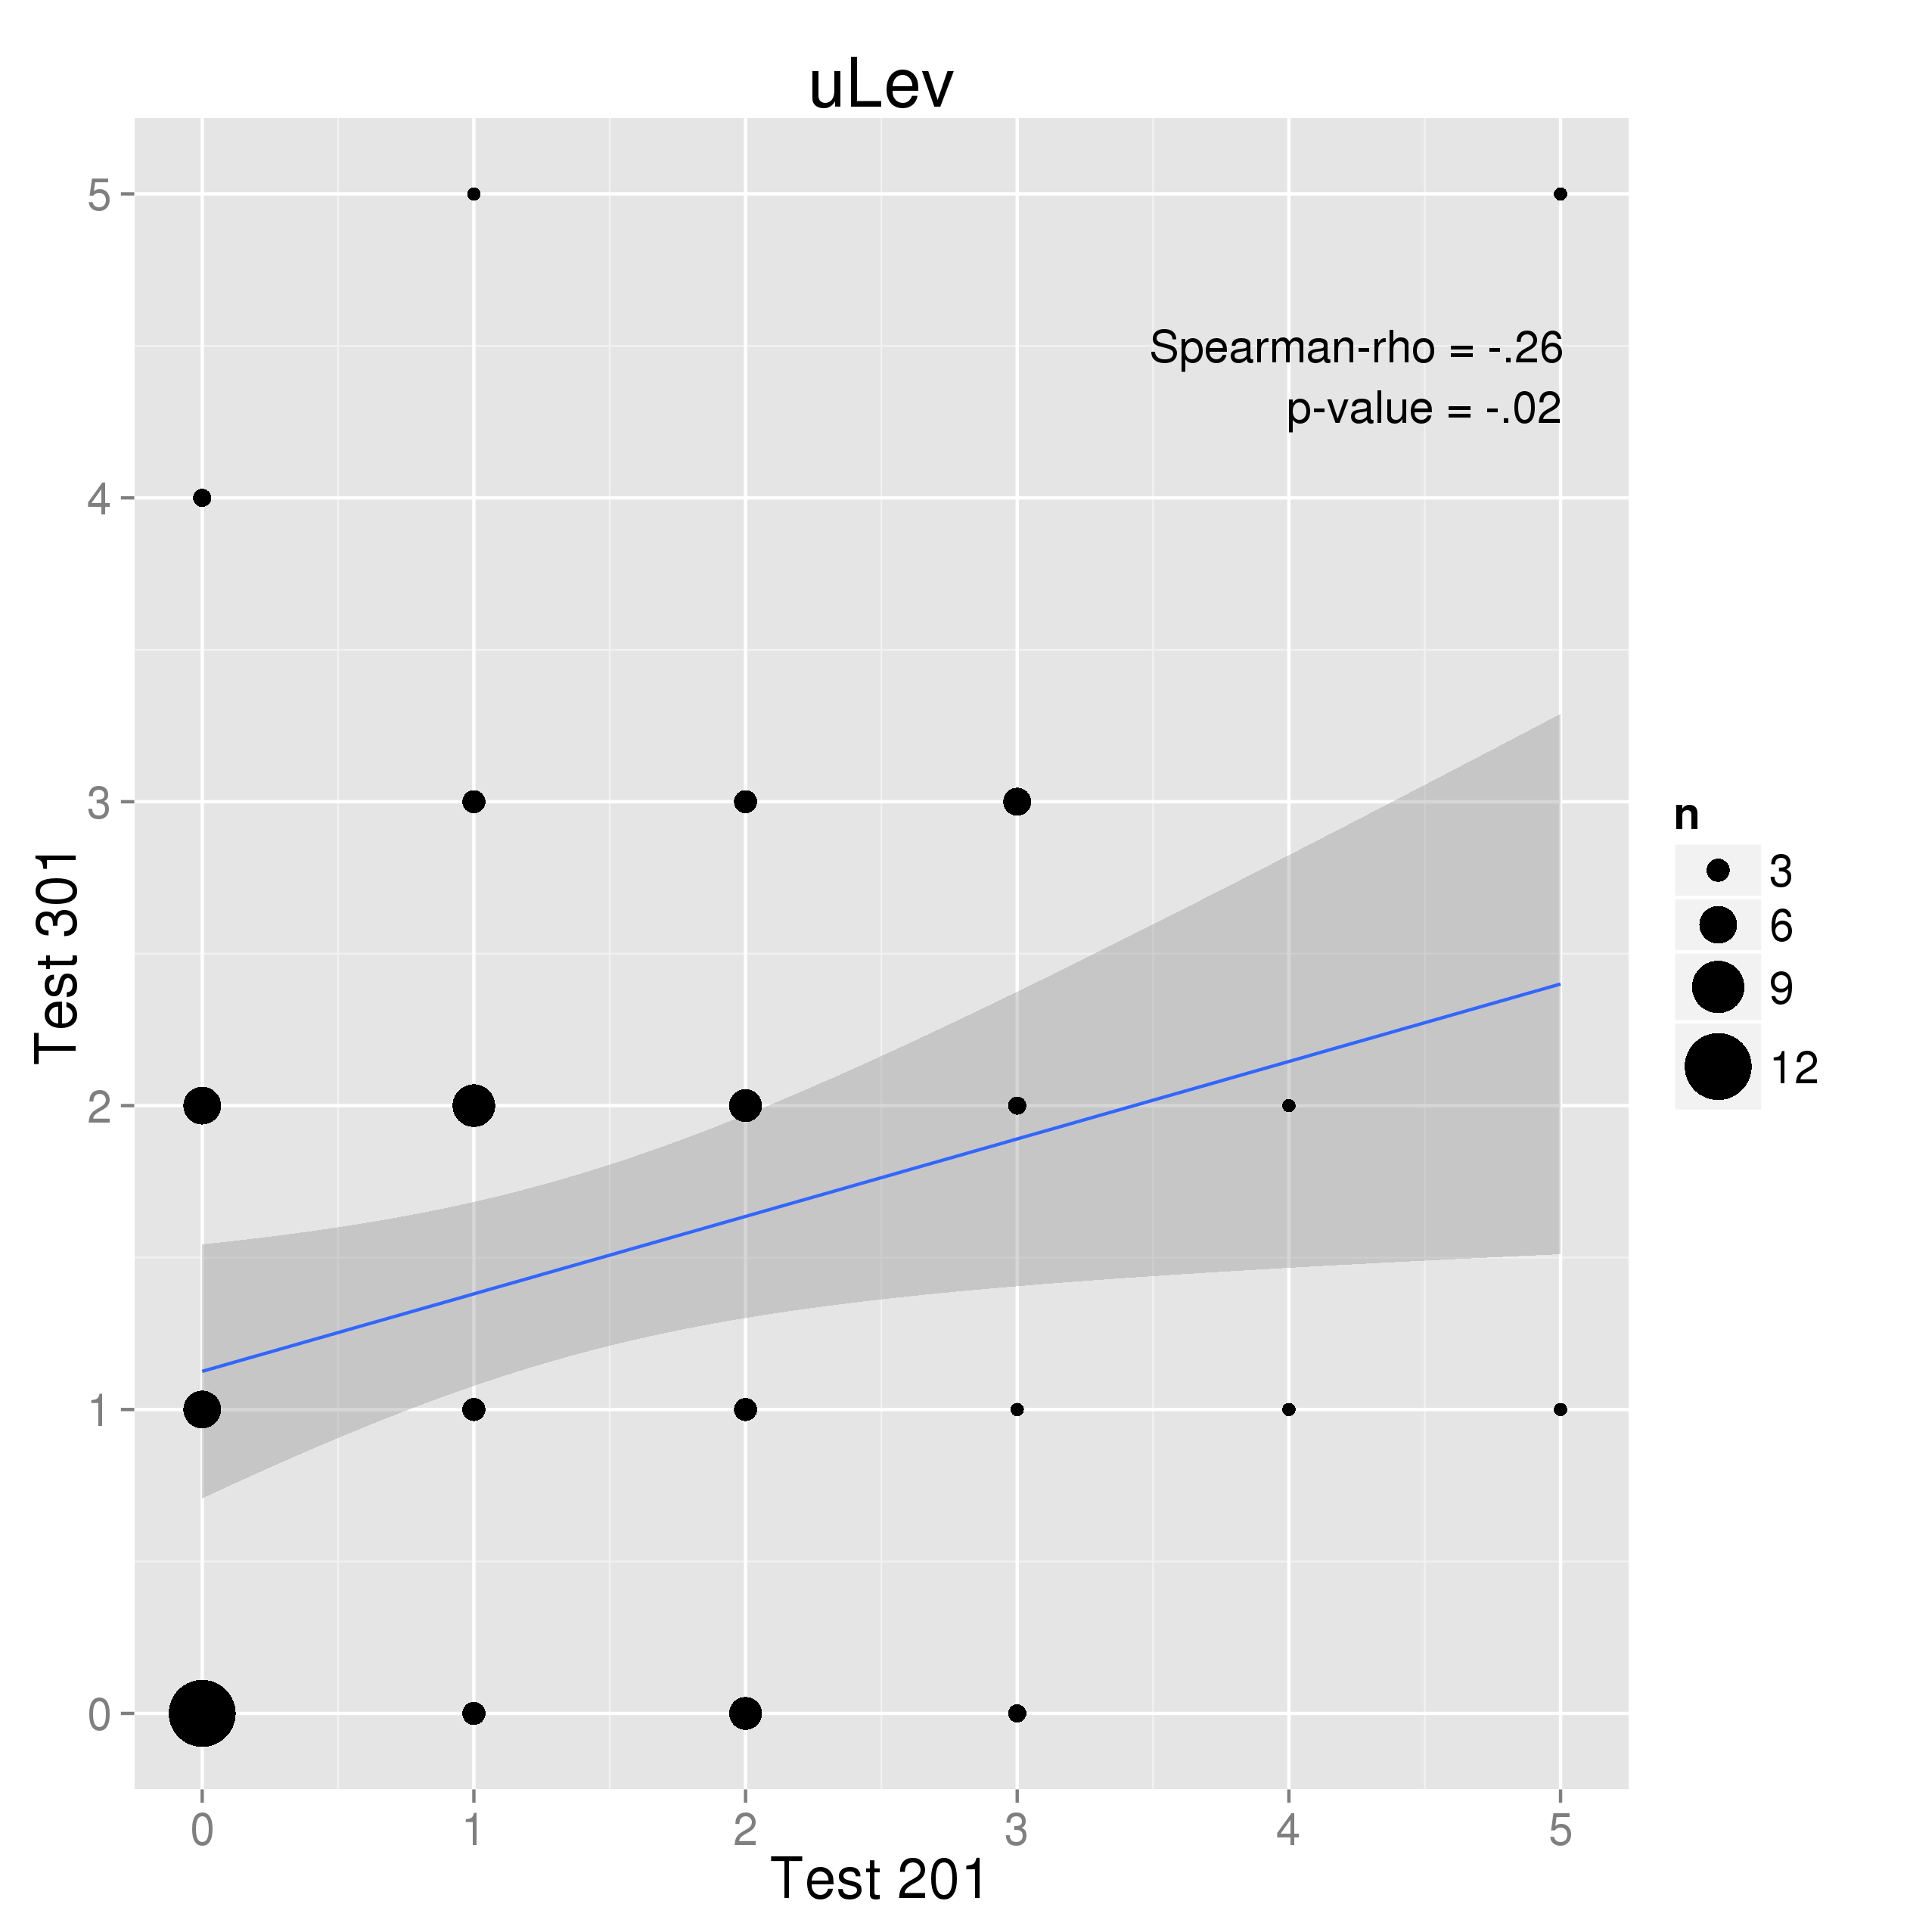
\includegraphics[width=1.0\linewidth]{graphics/cor201301u.png}
  \caption{unbedingte Niveau-Stufen}
  \label{fig:cor201301k}
\end{subfigure}
\begin{subfigure}{0.49\textwidth}
  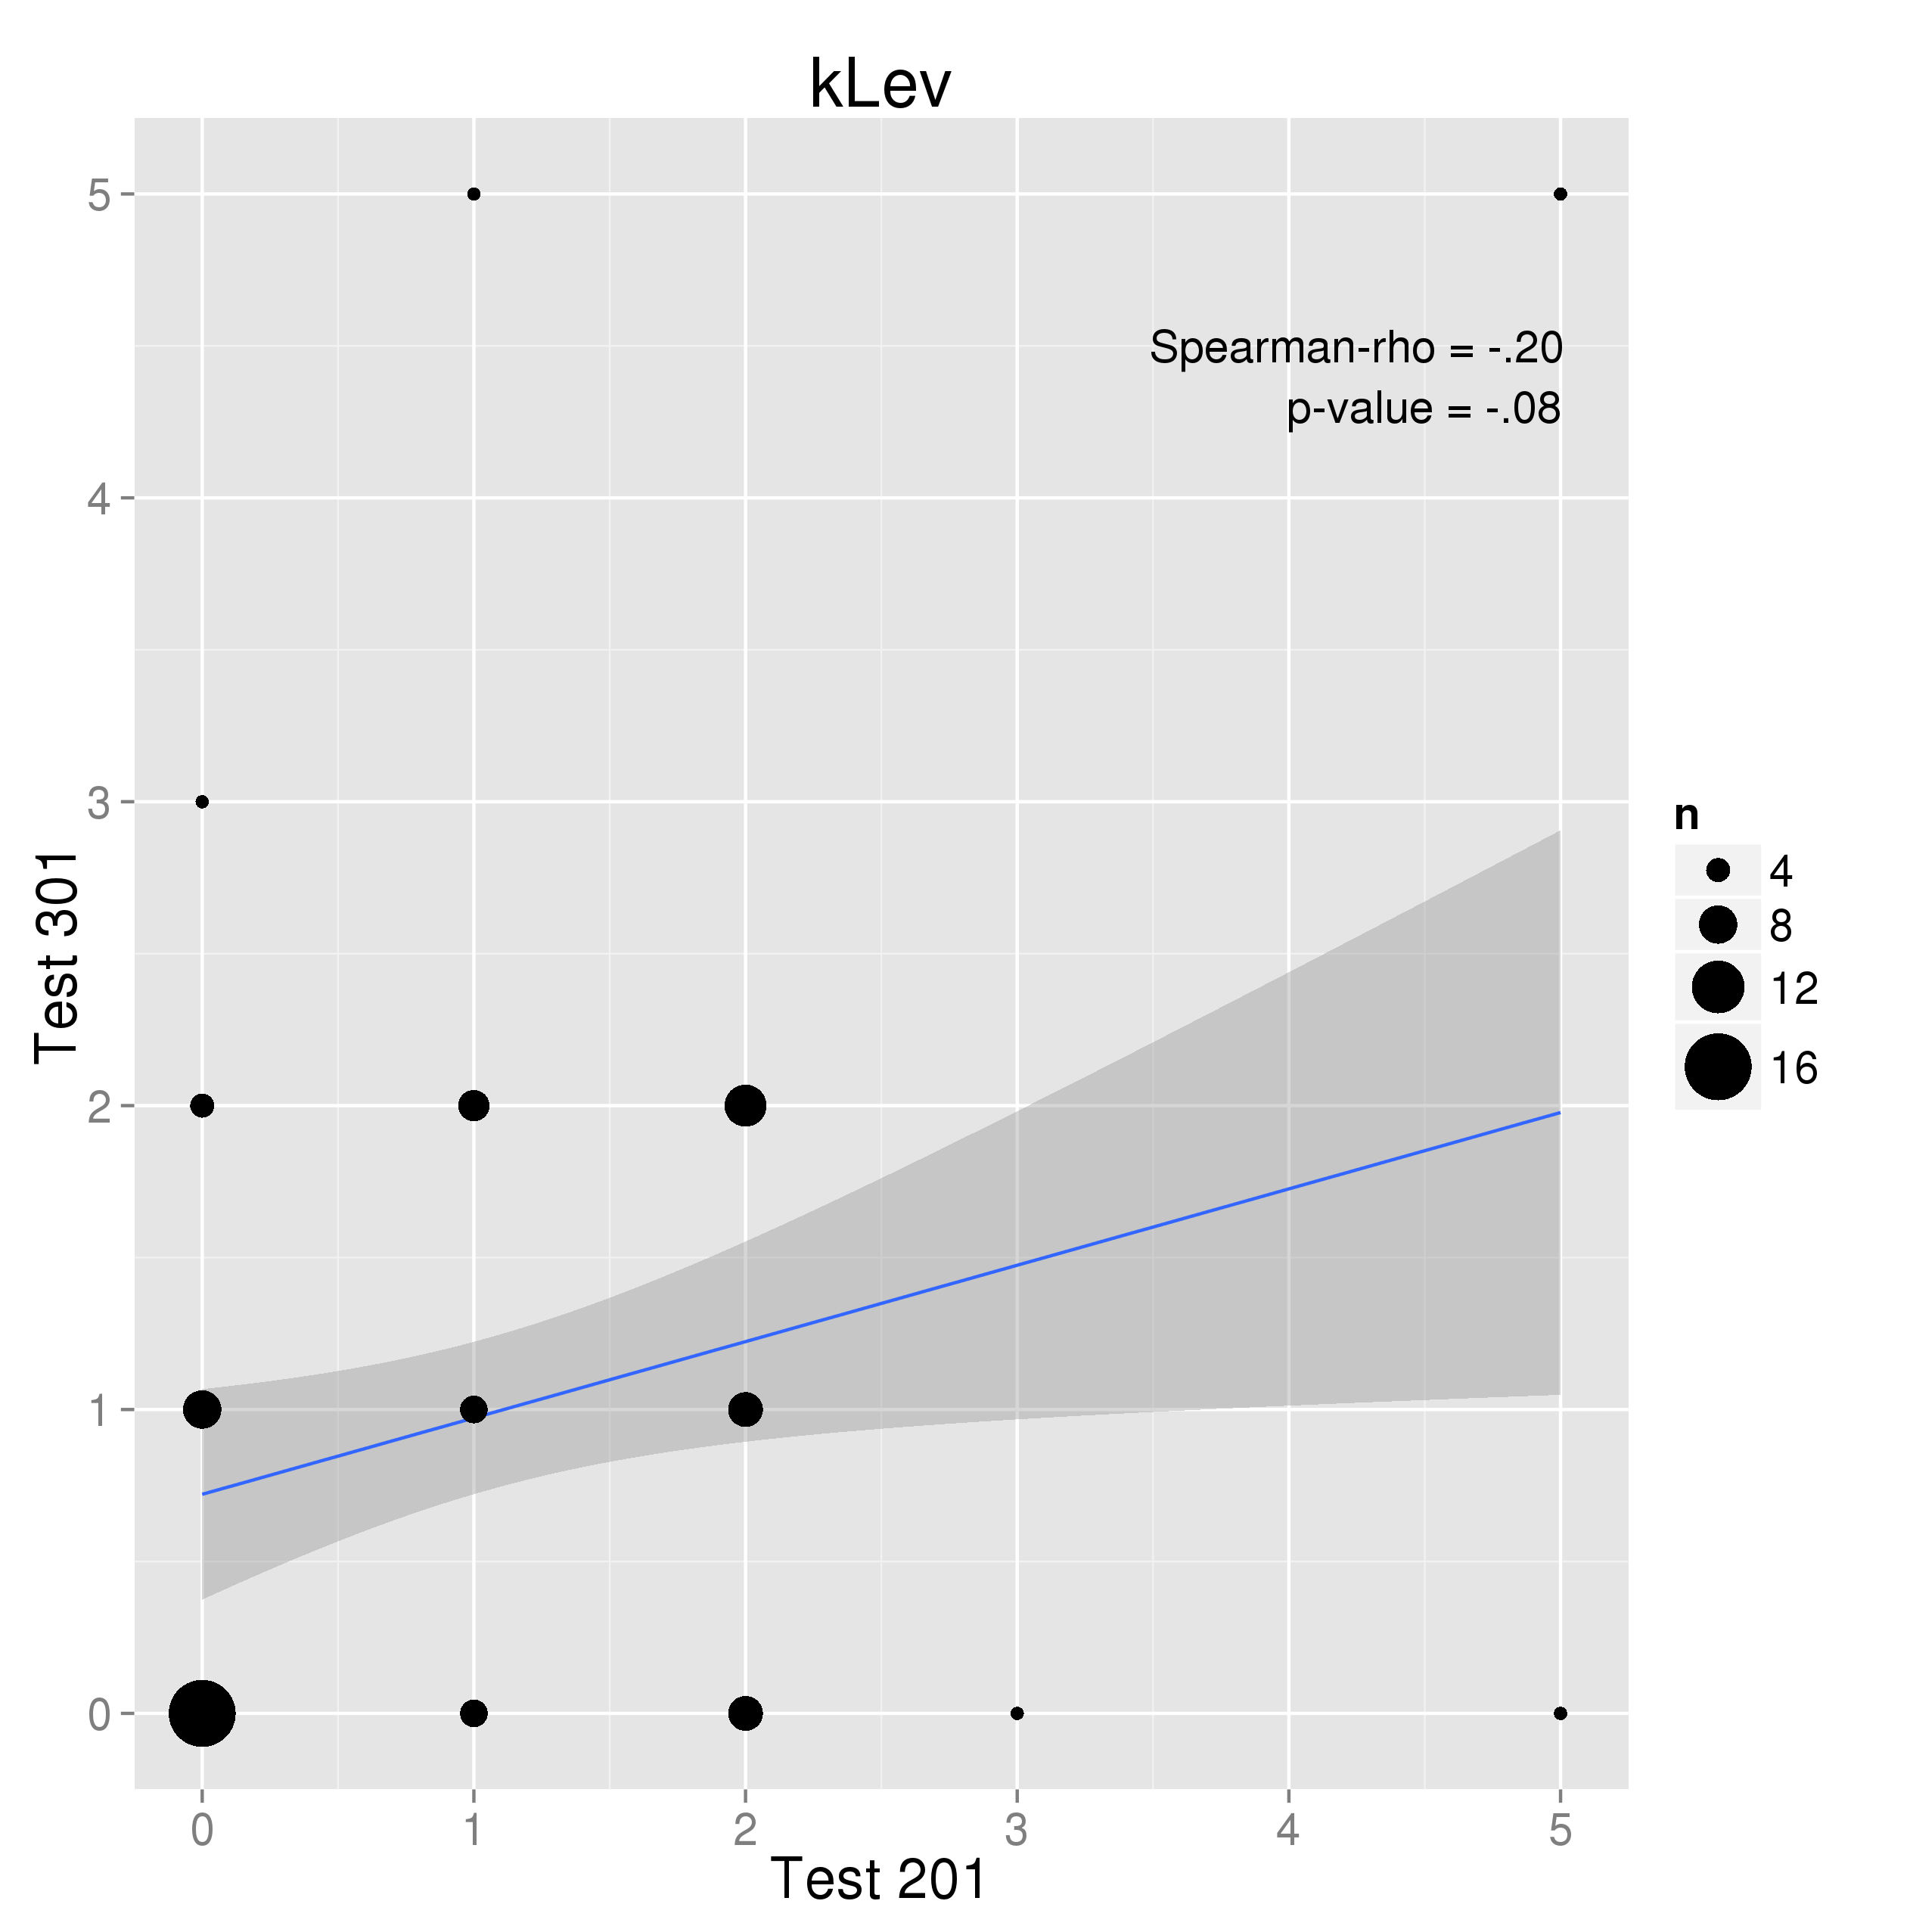
\includegraphics[width=1.0\linewidth]{graphics/cor201301k.png}
  \caption{bedingte Niveau-Stufen}
  \label{fig:cor201301u}
\end{subfigure}
\end{figure}
\begin{figure}[htbp]
\ContinuedFloat % continue from previous page
\centering
\begin{subfigure}{0.49\textwidth}
  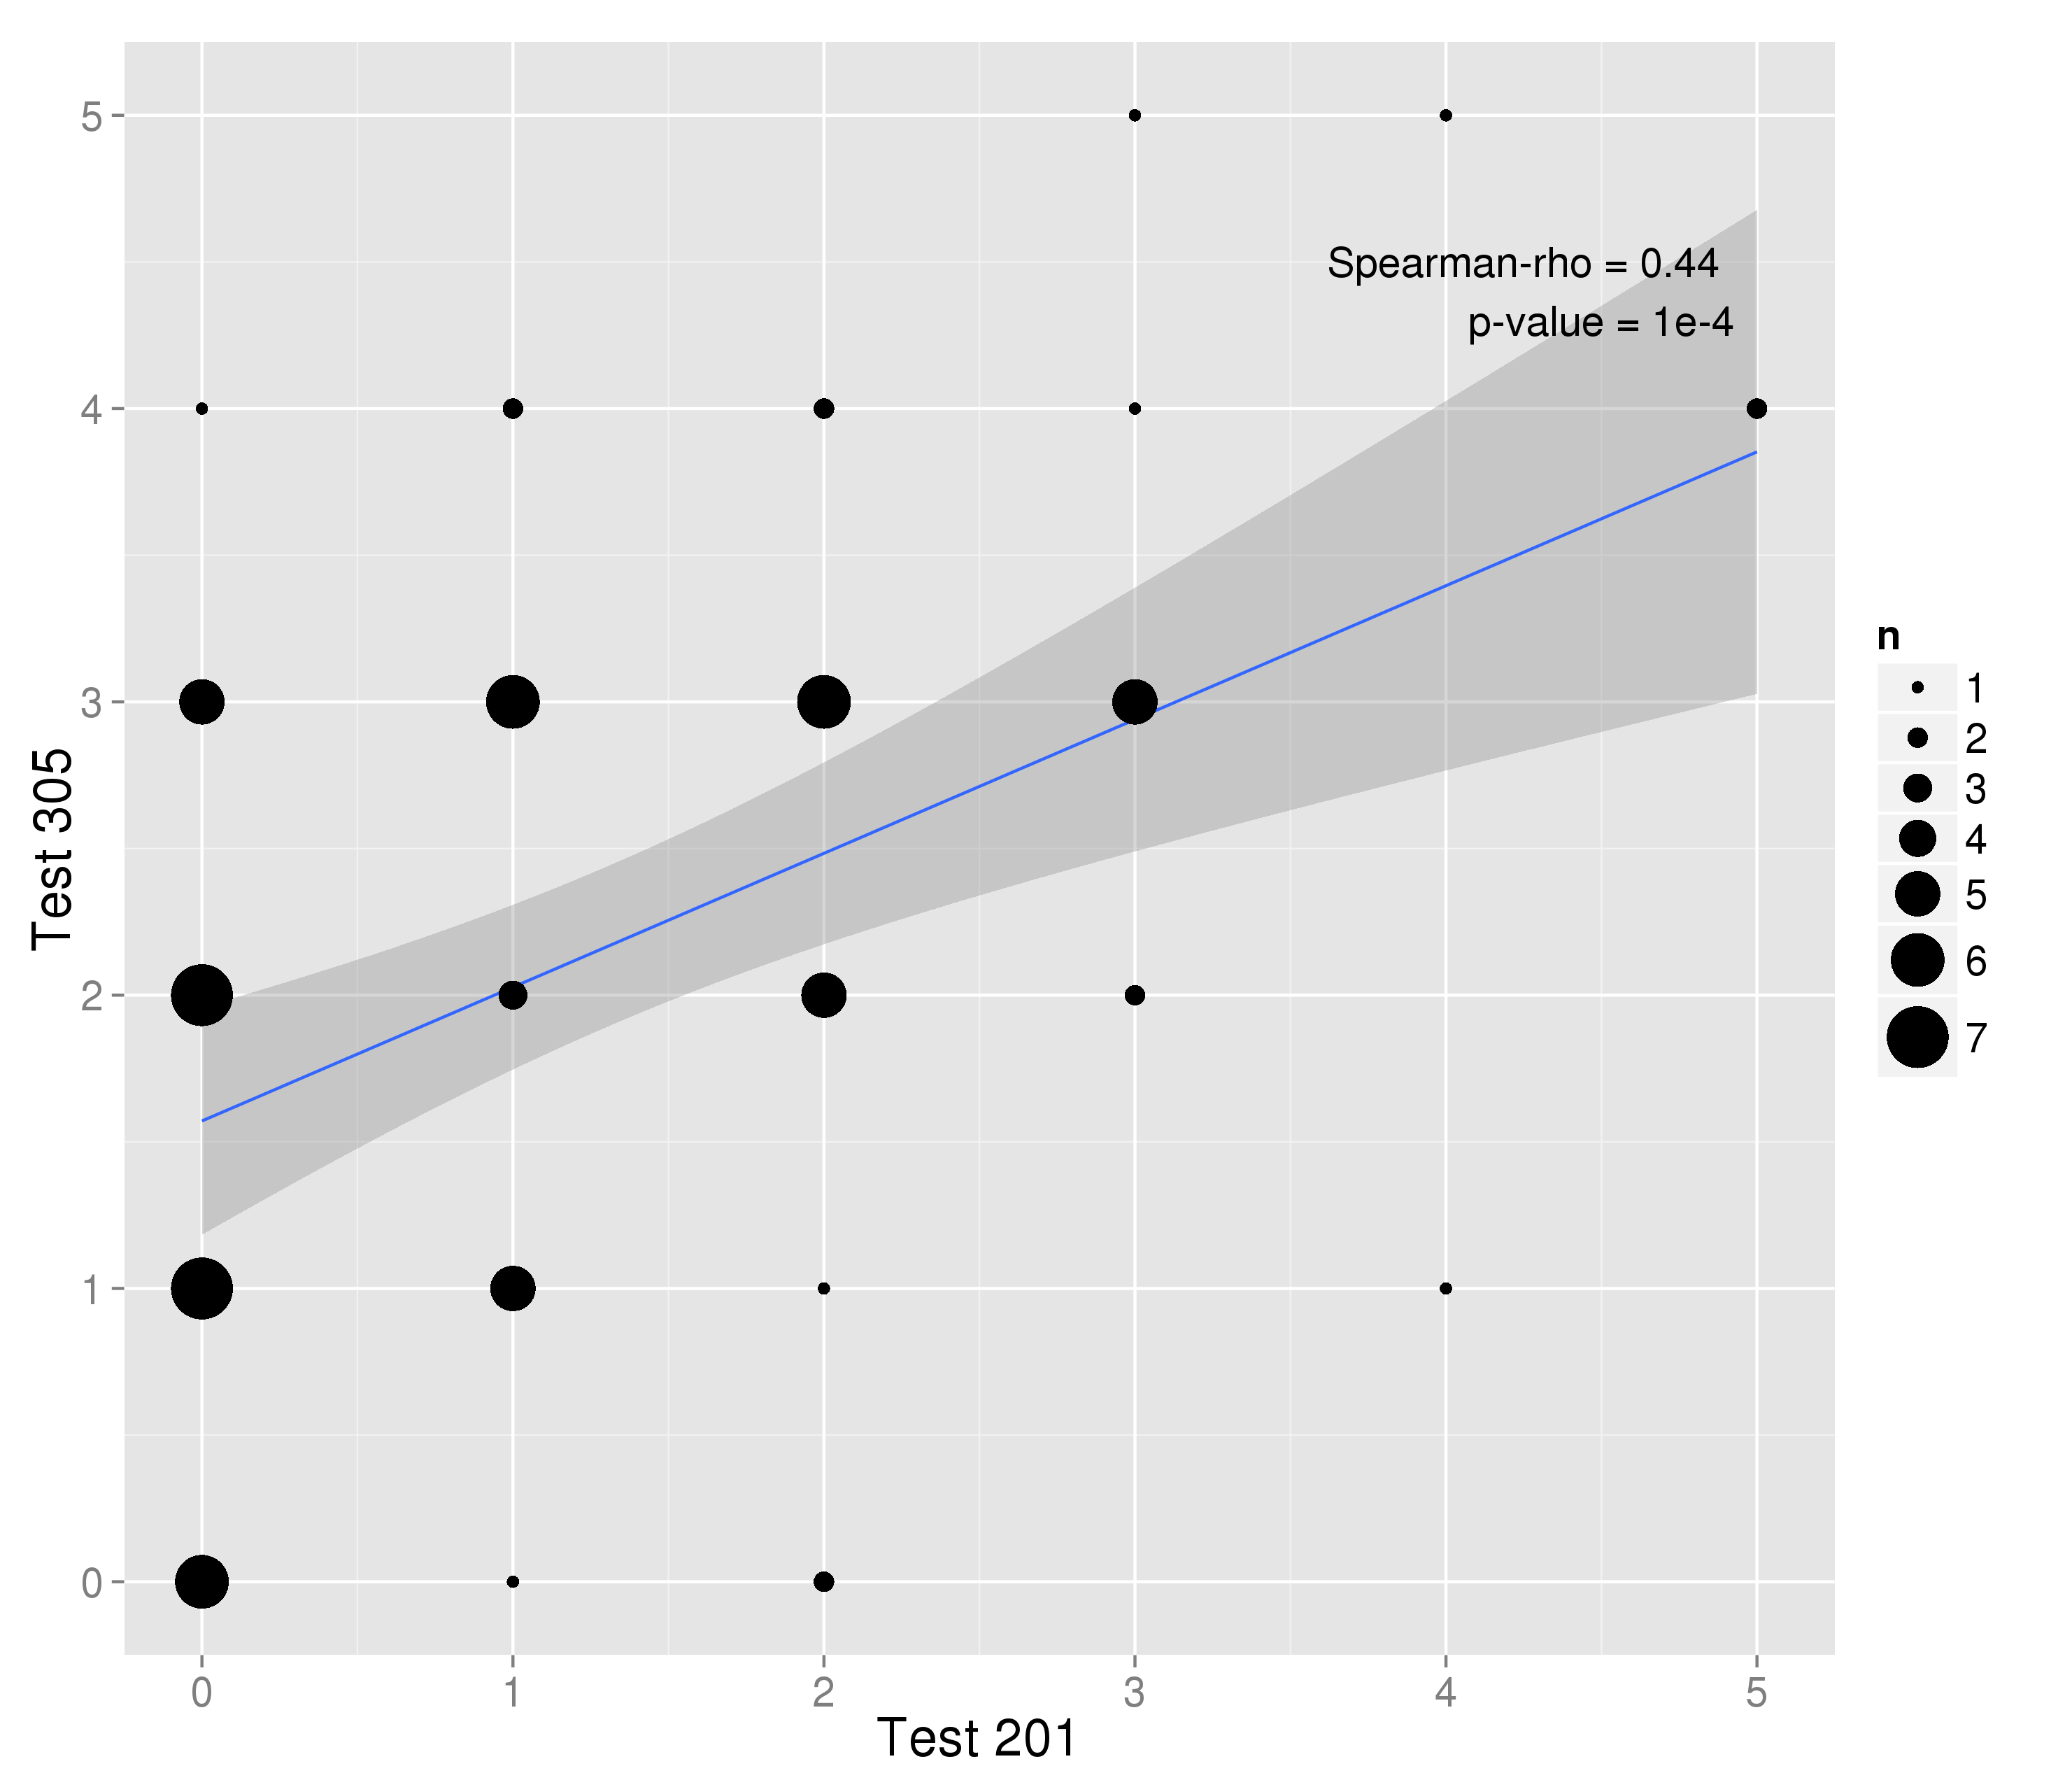
\includegraphics[width=1.0\linewidth]{graphics/cor201305u.png}
  \caption{unbedingte Niveau-Stufen}
  \label{fig:cor201305k}
\end{subfigure}
\begin{subfigure}{0.49\textwidth}
  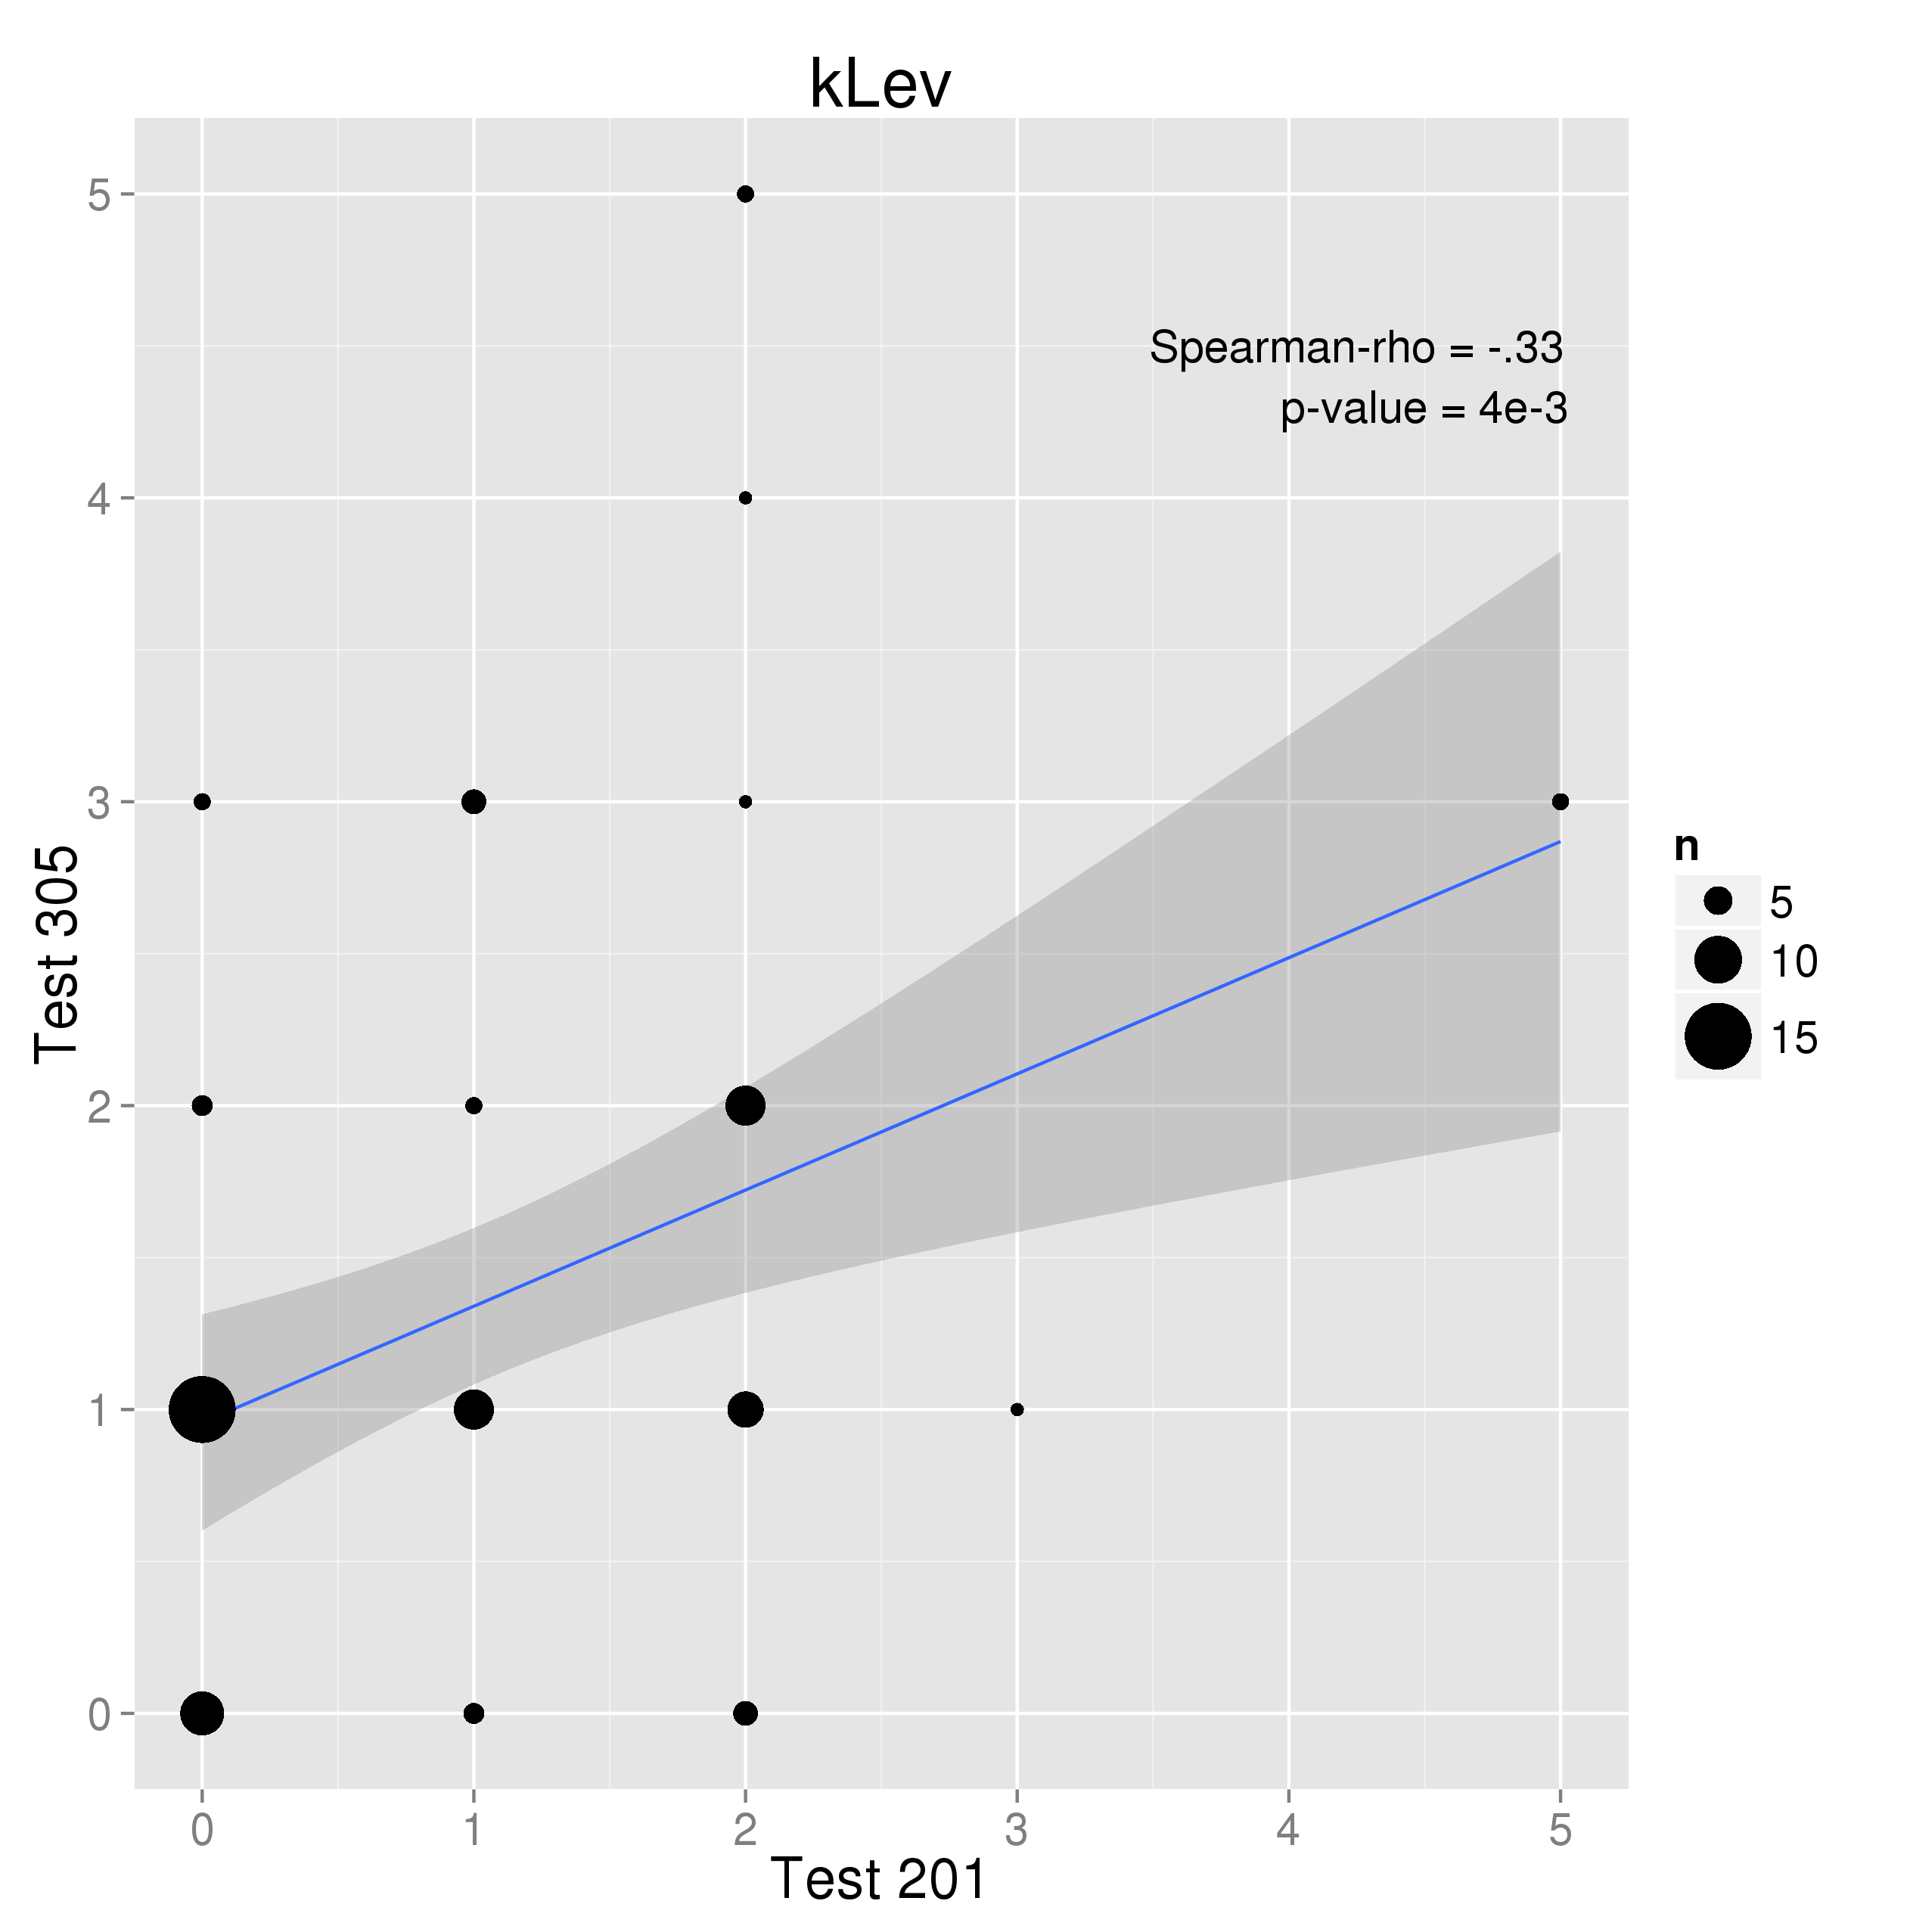
\includegraphics[width=1.0\linewidth]{graphics/cor201305k.png}
  \caption{bedingte Niveau-Stufen}
  \label{fig:cor201305u}
\end{subfigure}
\end{figure}
\begin{figure}[htbp]
\ContinuedFloat % continue from previous page
\centering
\begin{subfigure}{0.49\textwidth}
  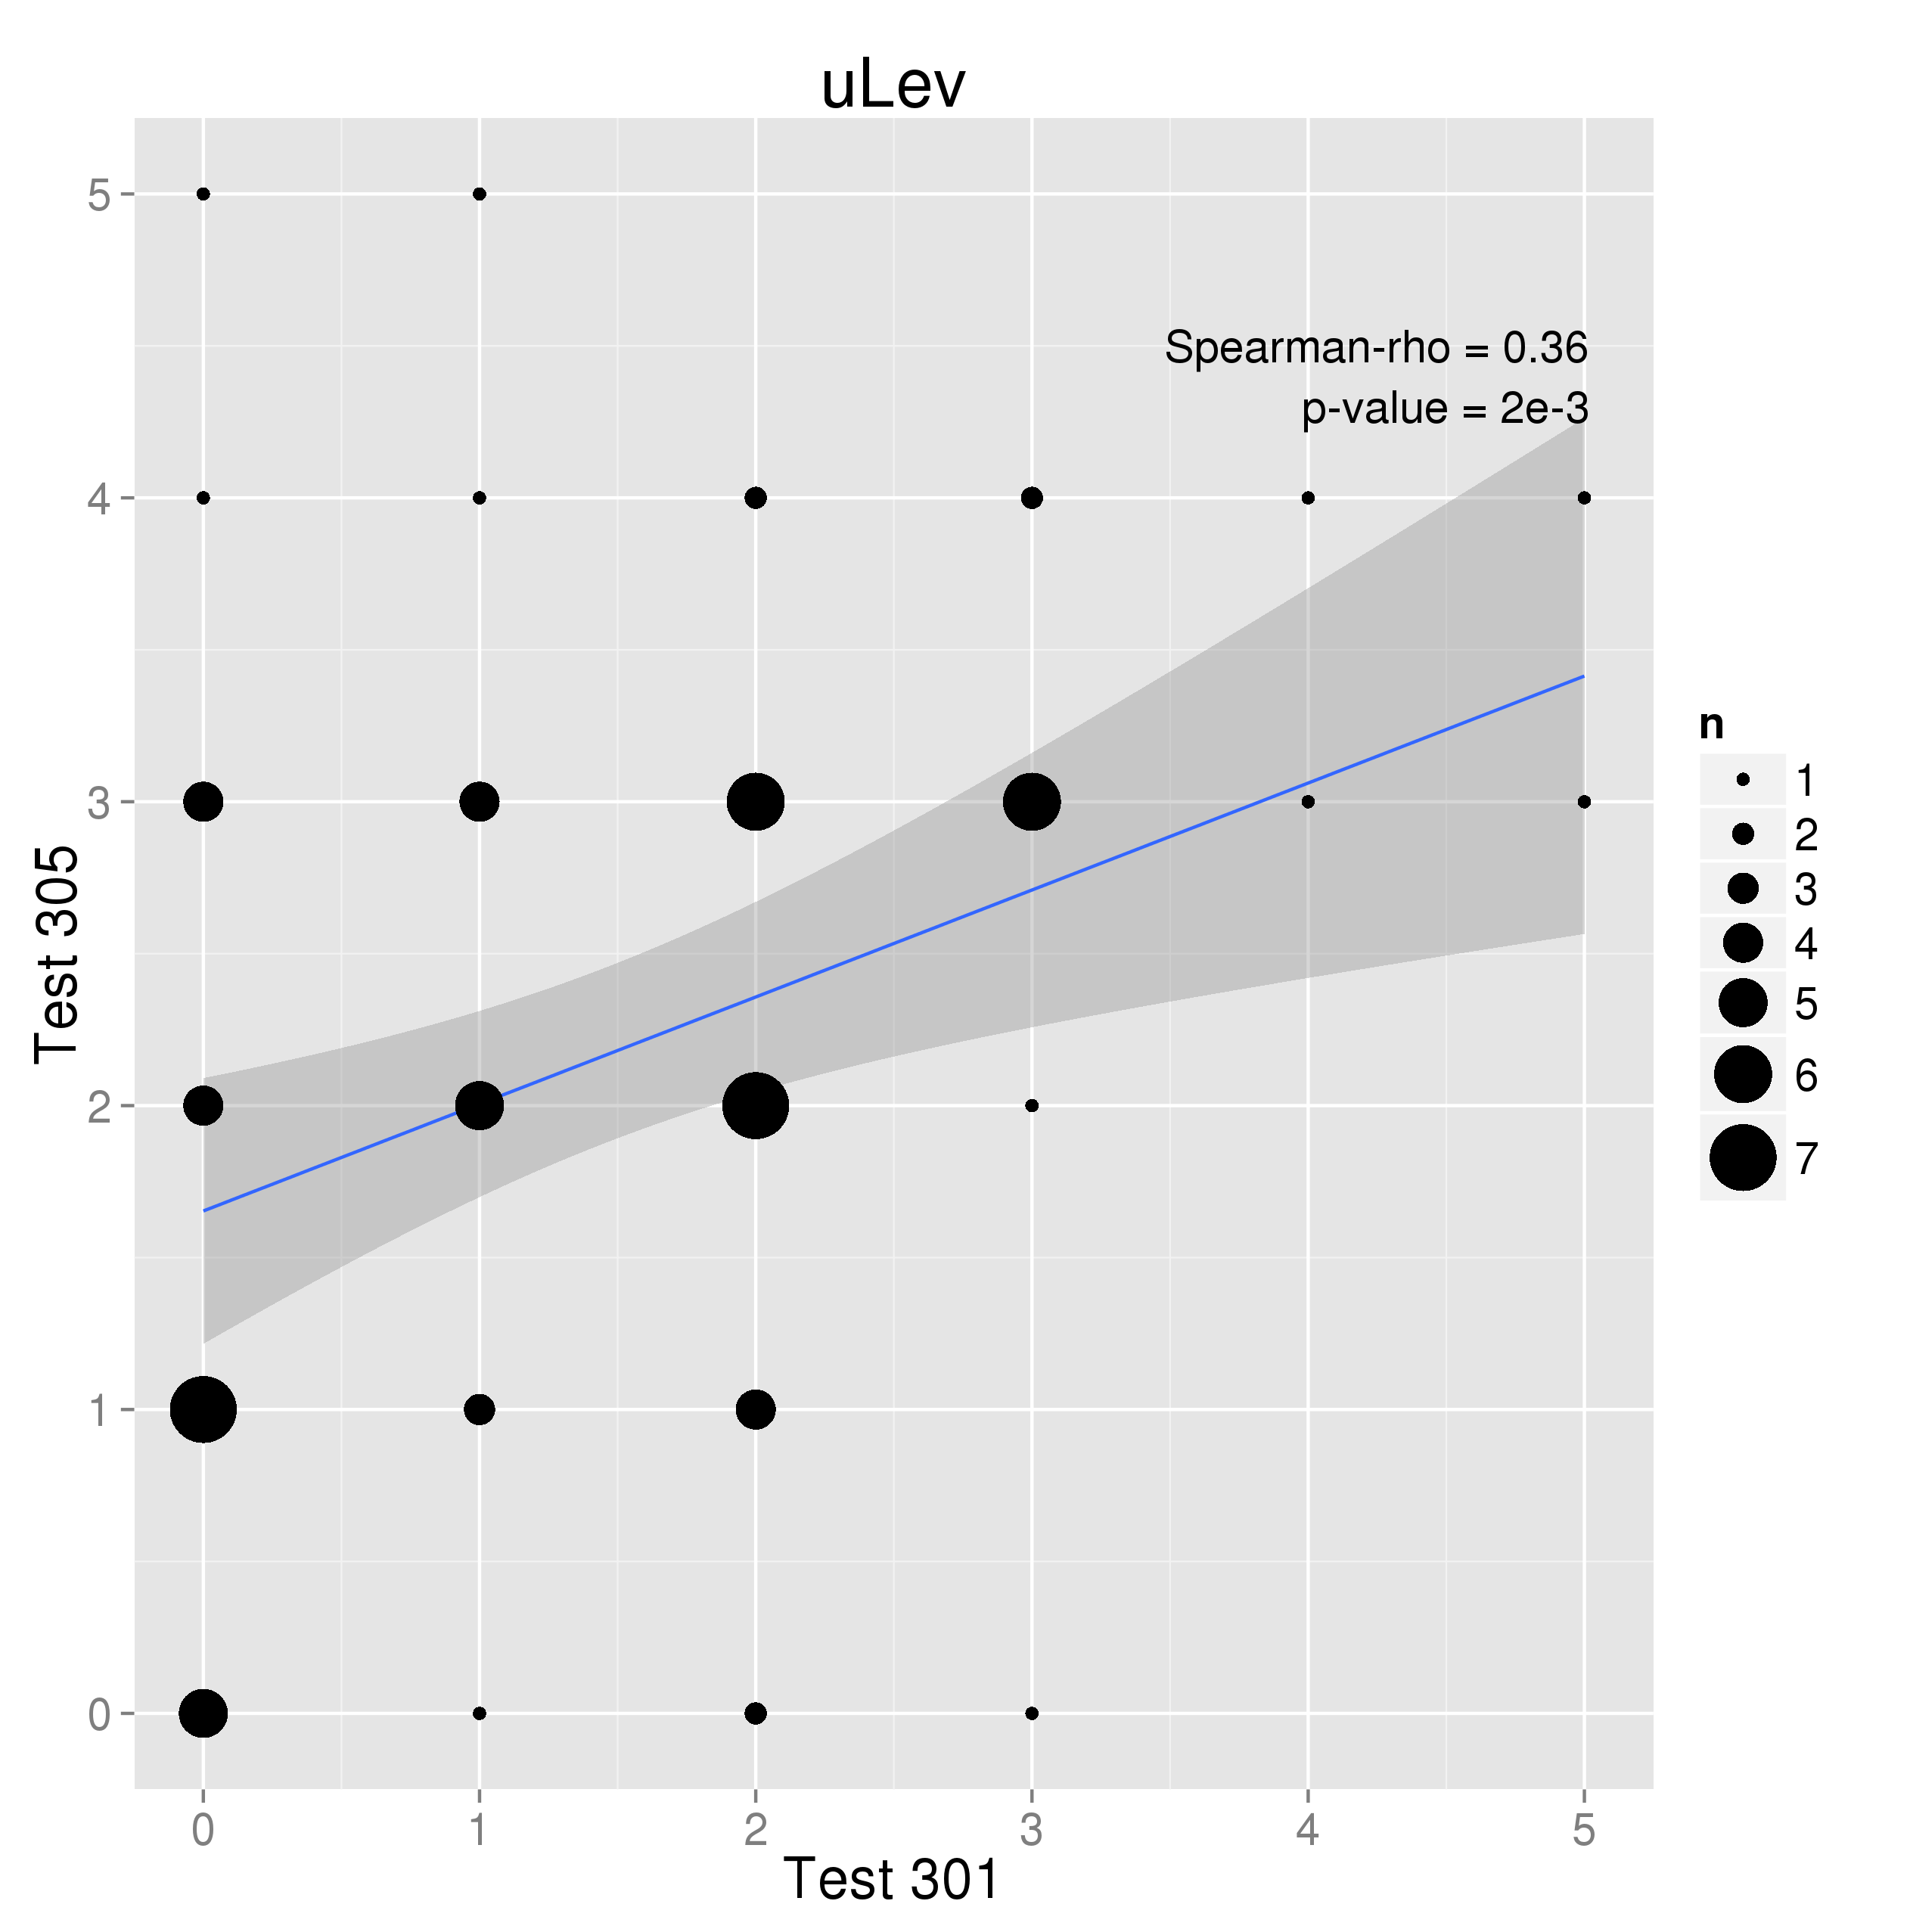
\includegraphics[width=1.0\linewidth]{graphics/cor301305u.png}
  \caption{unbedingte Niveau-Stufen}
  \label{fig:cor301305k}
\end{subfigure}
\begin{subfigure}{0.49\textwidth}
  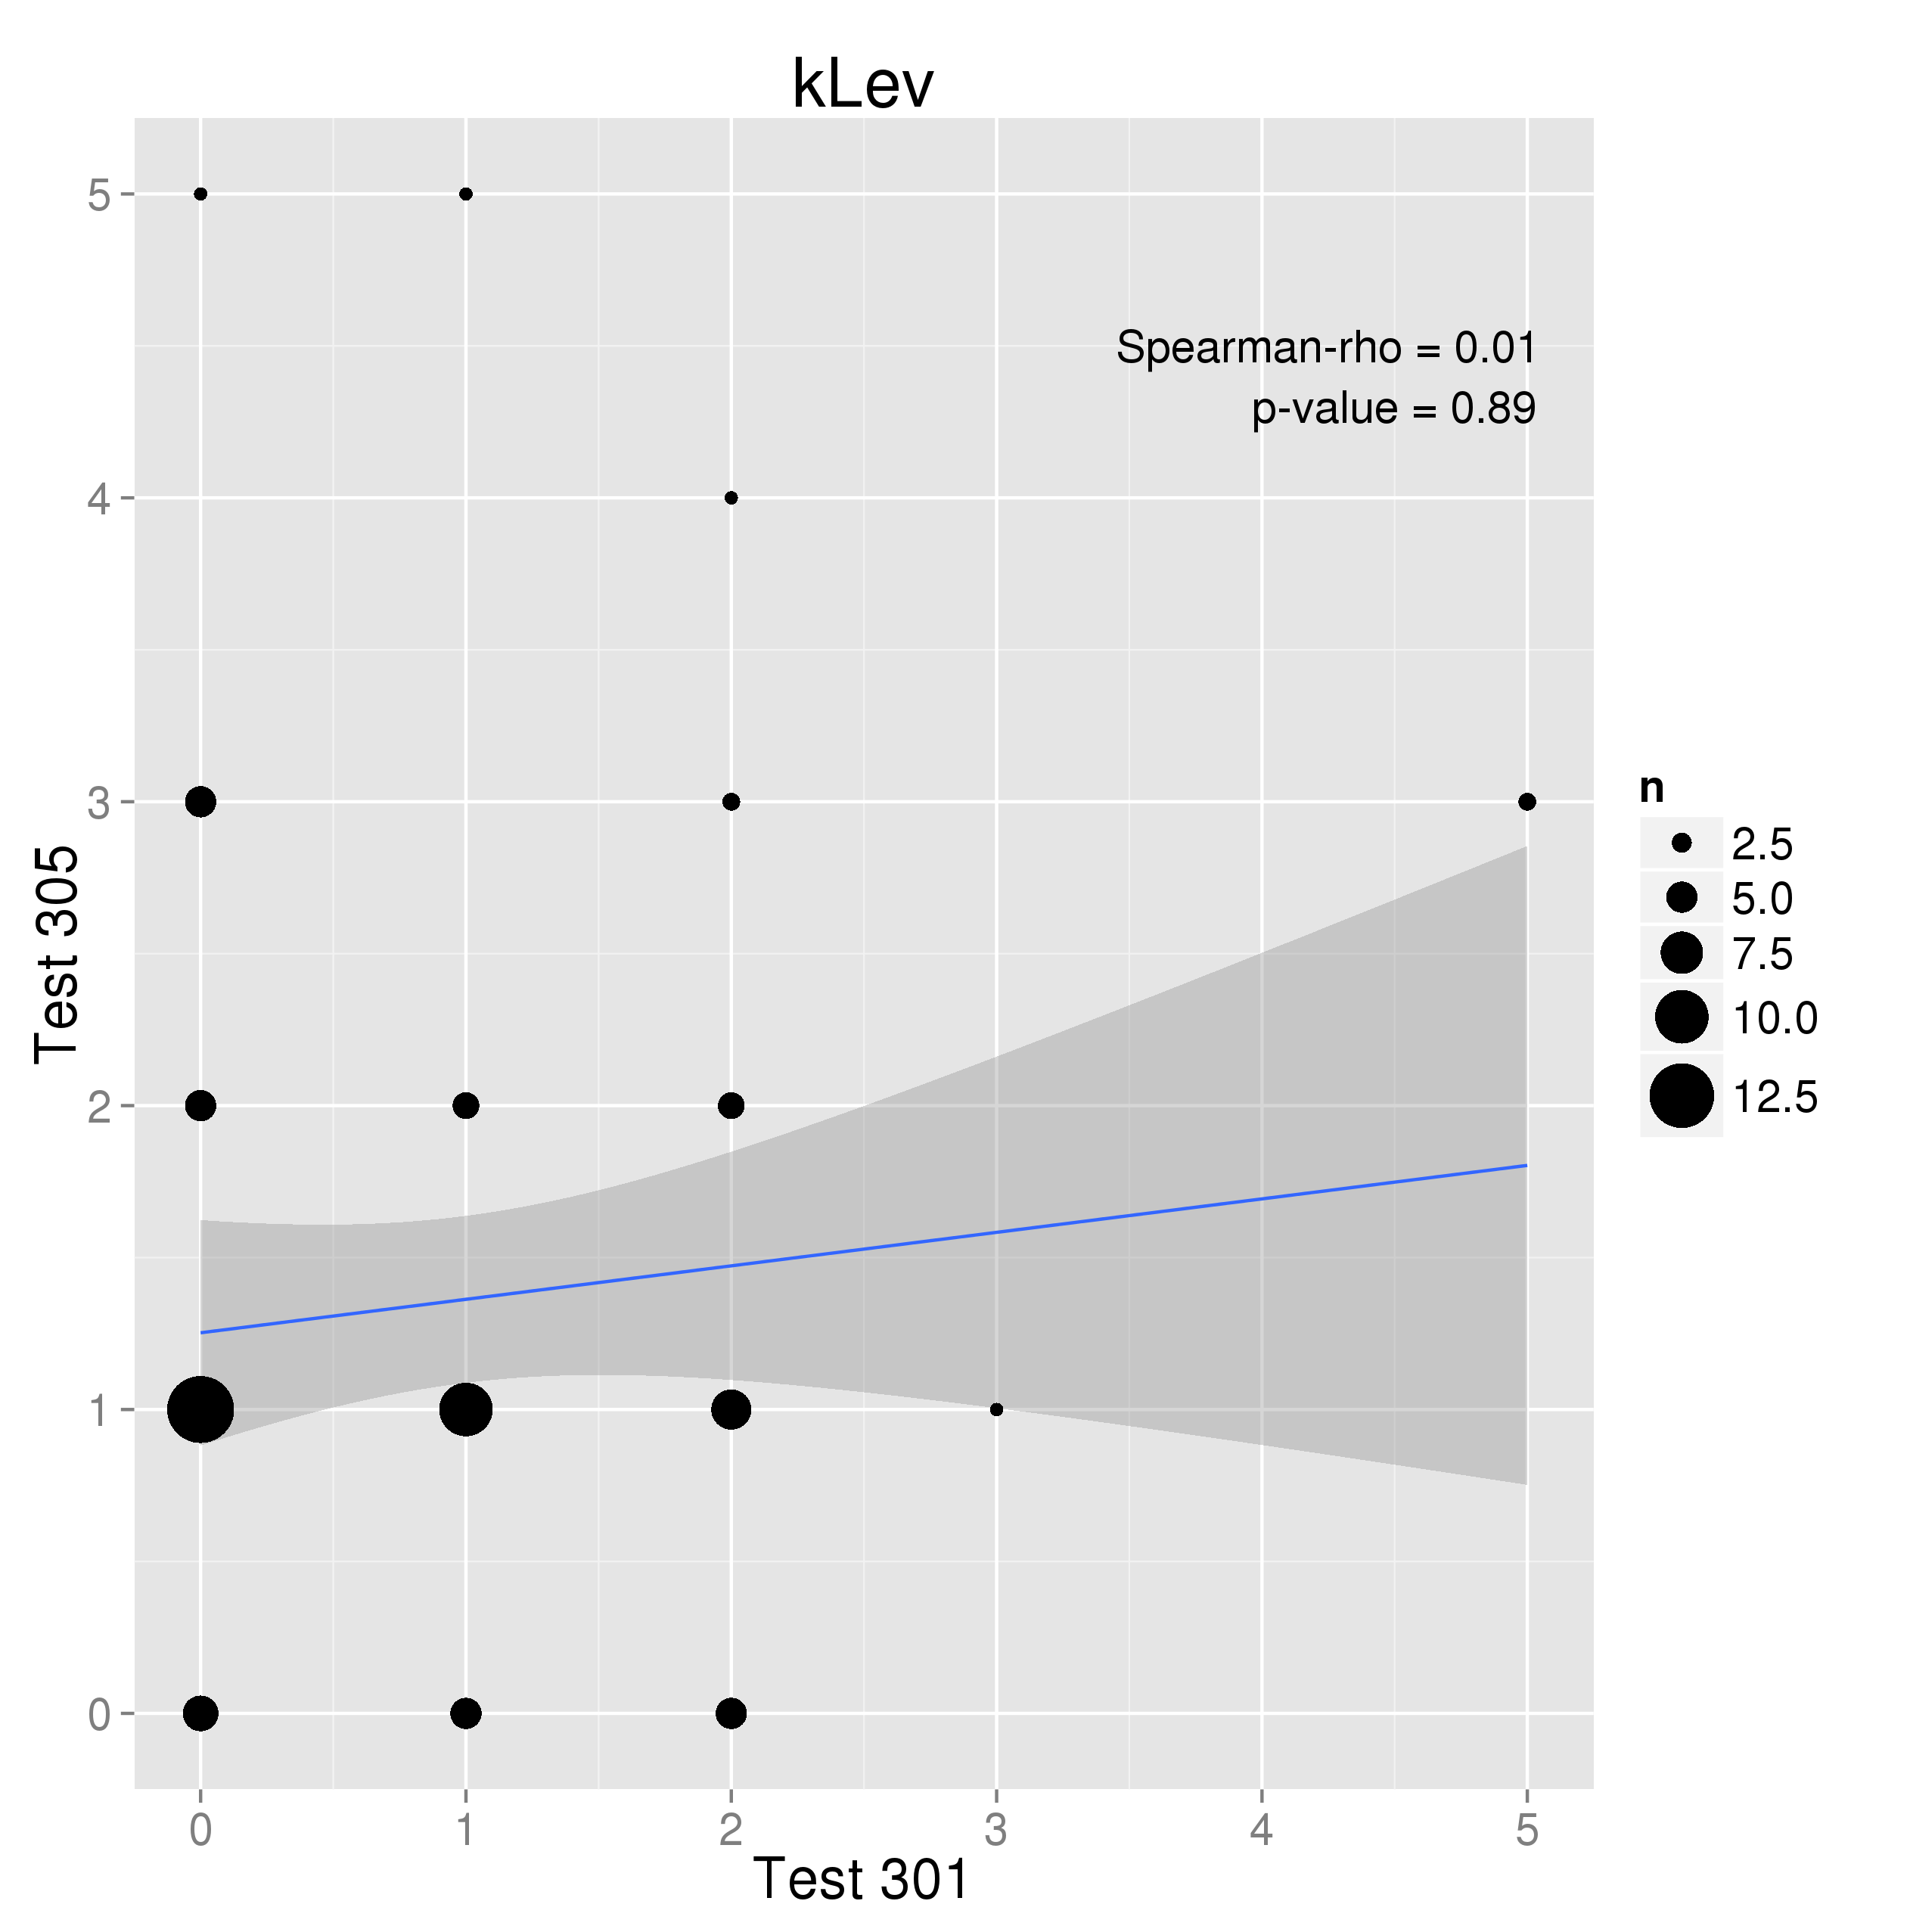
\includegraphics[width=1.0\linewidth]{graphics/cor301305k.png}
  \caption{bedingte Niveau-Stufen}
  \label{fig:cor301305u}
\end{subfigure}

\caption{Korrelation zwischen den Niveau Stufen zwischen den einzelnen Tests. Der Durchmesser der Punkte ist ein Mass für die Anzahl an Datenpunkten, welche an dieser Position liegen. Die blaue Gerade ist die lineare Regression der zugrunde liegenden Daten, der dunkel graue Bereich stellt das Vertrauensintervall (95\%) der linearen Regression dar. Zusätzlich sind noch Spearmans $rho$ und der p-Wert des Signifikanztests angegeben.}
\label{fig:corLev}
\end{figure}

\github{http://git.io/FnbD}


\section{Rasch-Analyse}

Als Probabilistische Test-Methode wurde das Rasch Modell verwendet. Der Grund für diese Methodik war, dass es sich bei der Kompetenz des skalenbasierten Messens um ein latentes Merkmal handelt. In anderen Worten die Kompetenz des skalenbaiserten Messens ist nicht direkt beobachtbar.

Es wurde zuerst folgendes Rasch Modell verwendet.

\begin{eqnarray}
P(U_{ij}=u_{ij}|\theta_i,\beta_j) = \frac{e^{u_{ij}(\theta_i-\beta_j)}}{1+e^{\theta_i-\beta_j}}
\end{eqnarray}

Wobei i=1,…,n die Zählvariable für eine Person ist und j=1,…,m die Zählvariable für eine Aufgabe darstellt. Die Variable $u_{ij} \in \{0,1\}$ die dichotome Antwort einer Person auf eine Frage ist. Die Variable $\beta_j$ beschreibt den Schwierigkeitsgrad einer Aufgabe und $\theta_j$ die latente Fähigkeit einer Person.

Bei der Item-Response-Theorie (Probabilistische Test-Methoden) wird angenommen , dass das Ergebnis einer Person nicht deterministisch ist, sondern zufällig sein kann. Daher soll mit dem Rasch Modell die Lösungswahrscheinlichkeit jeder Aufgabe $U_{ij}$ berechnet werden. Diese Lösungswahrscheinlichkeit hängt sowohl von der Fähigkeit der Person $\theta_j$ als auch von der Schwierigkeit der Aufgabe $\beta_i$ ab. Diese Lösungswahrscheinlichkeiten werden basierend auf den Testergebnissen $u_{ij}$ geschätzt.

\subsection{Parameterschätzung}
Für die Parameterschätzung gibt es verschieden Ansätze. Da die beste Methode von den Daten abhängig ist wurde in einem ersten Schritt das Rasch-Modell sowohl mit der bedingte Maximum-Likelihood-Schätzung, als auch mit der marginal Maximum-Likelihood-Schätzung getestet und die Resultate wurden verglichen. 

Bei der bedingten Maximum-Likelihood-Schätzung wird ein zweistufiges Vorgehen gewählt. Zuerst werden die Aufgaben-Parameter geschätzt ohne die Personen Parameter zu beachten. Erst in einem zweiten Schritt werden die Personen-Parameter geschätzt. Ein Problem dieser Methodik ist, dass Personenfertigkeiten von Personen, welche keine oder alle Aufgaben gelöst haben nicht geschätzt werden können \citep{Mair2007}.

In der marginalen Maximum-Likelihood-Schätzung wird angenommen, dass für die Personenfähigkeiten in der Stichprobe eine Normalverteilung vorliegt. Diese Annahme ist insbesondere dann problematisch, wenn nur eine Stichprobe der Gesamtbevölkerung verwendet wird \citep{Rizopoulos2006}.

Da beide Schätzungen für den vorliegenden Datensatz problematisch sein könnten, wurde das Rasch-Modell mit beiden Ansätzen durchgeführt und die Resultate verglichen. Das Ziel war dabei, den besseren Ansatz für den vorliegenden Datensatz zu finden, um mit diesem Ansatz die weiteren Analysen durchzuführen. Als Datensatz für diesen Vergleich wurden die 15 unbedingten Qualitätsstandards verwendet. Die Resultate sind in Abbildung \ref{fig:RaschVergleich} ersichtlich. Es gibt für diesen Datensatz keinerlei Unterschied in beiden Parameterschätzern.


\begin{figure}[htbp]

\centering
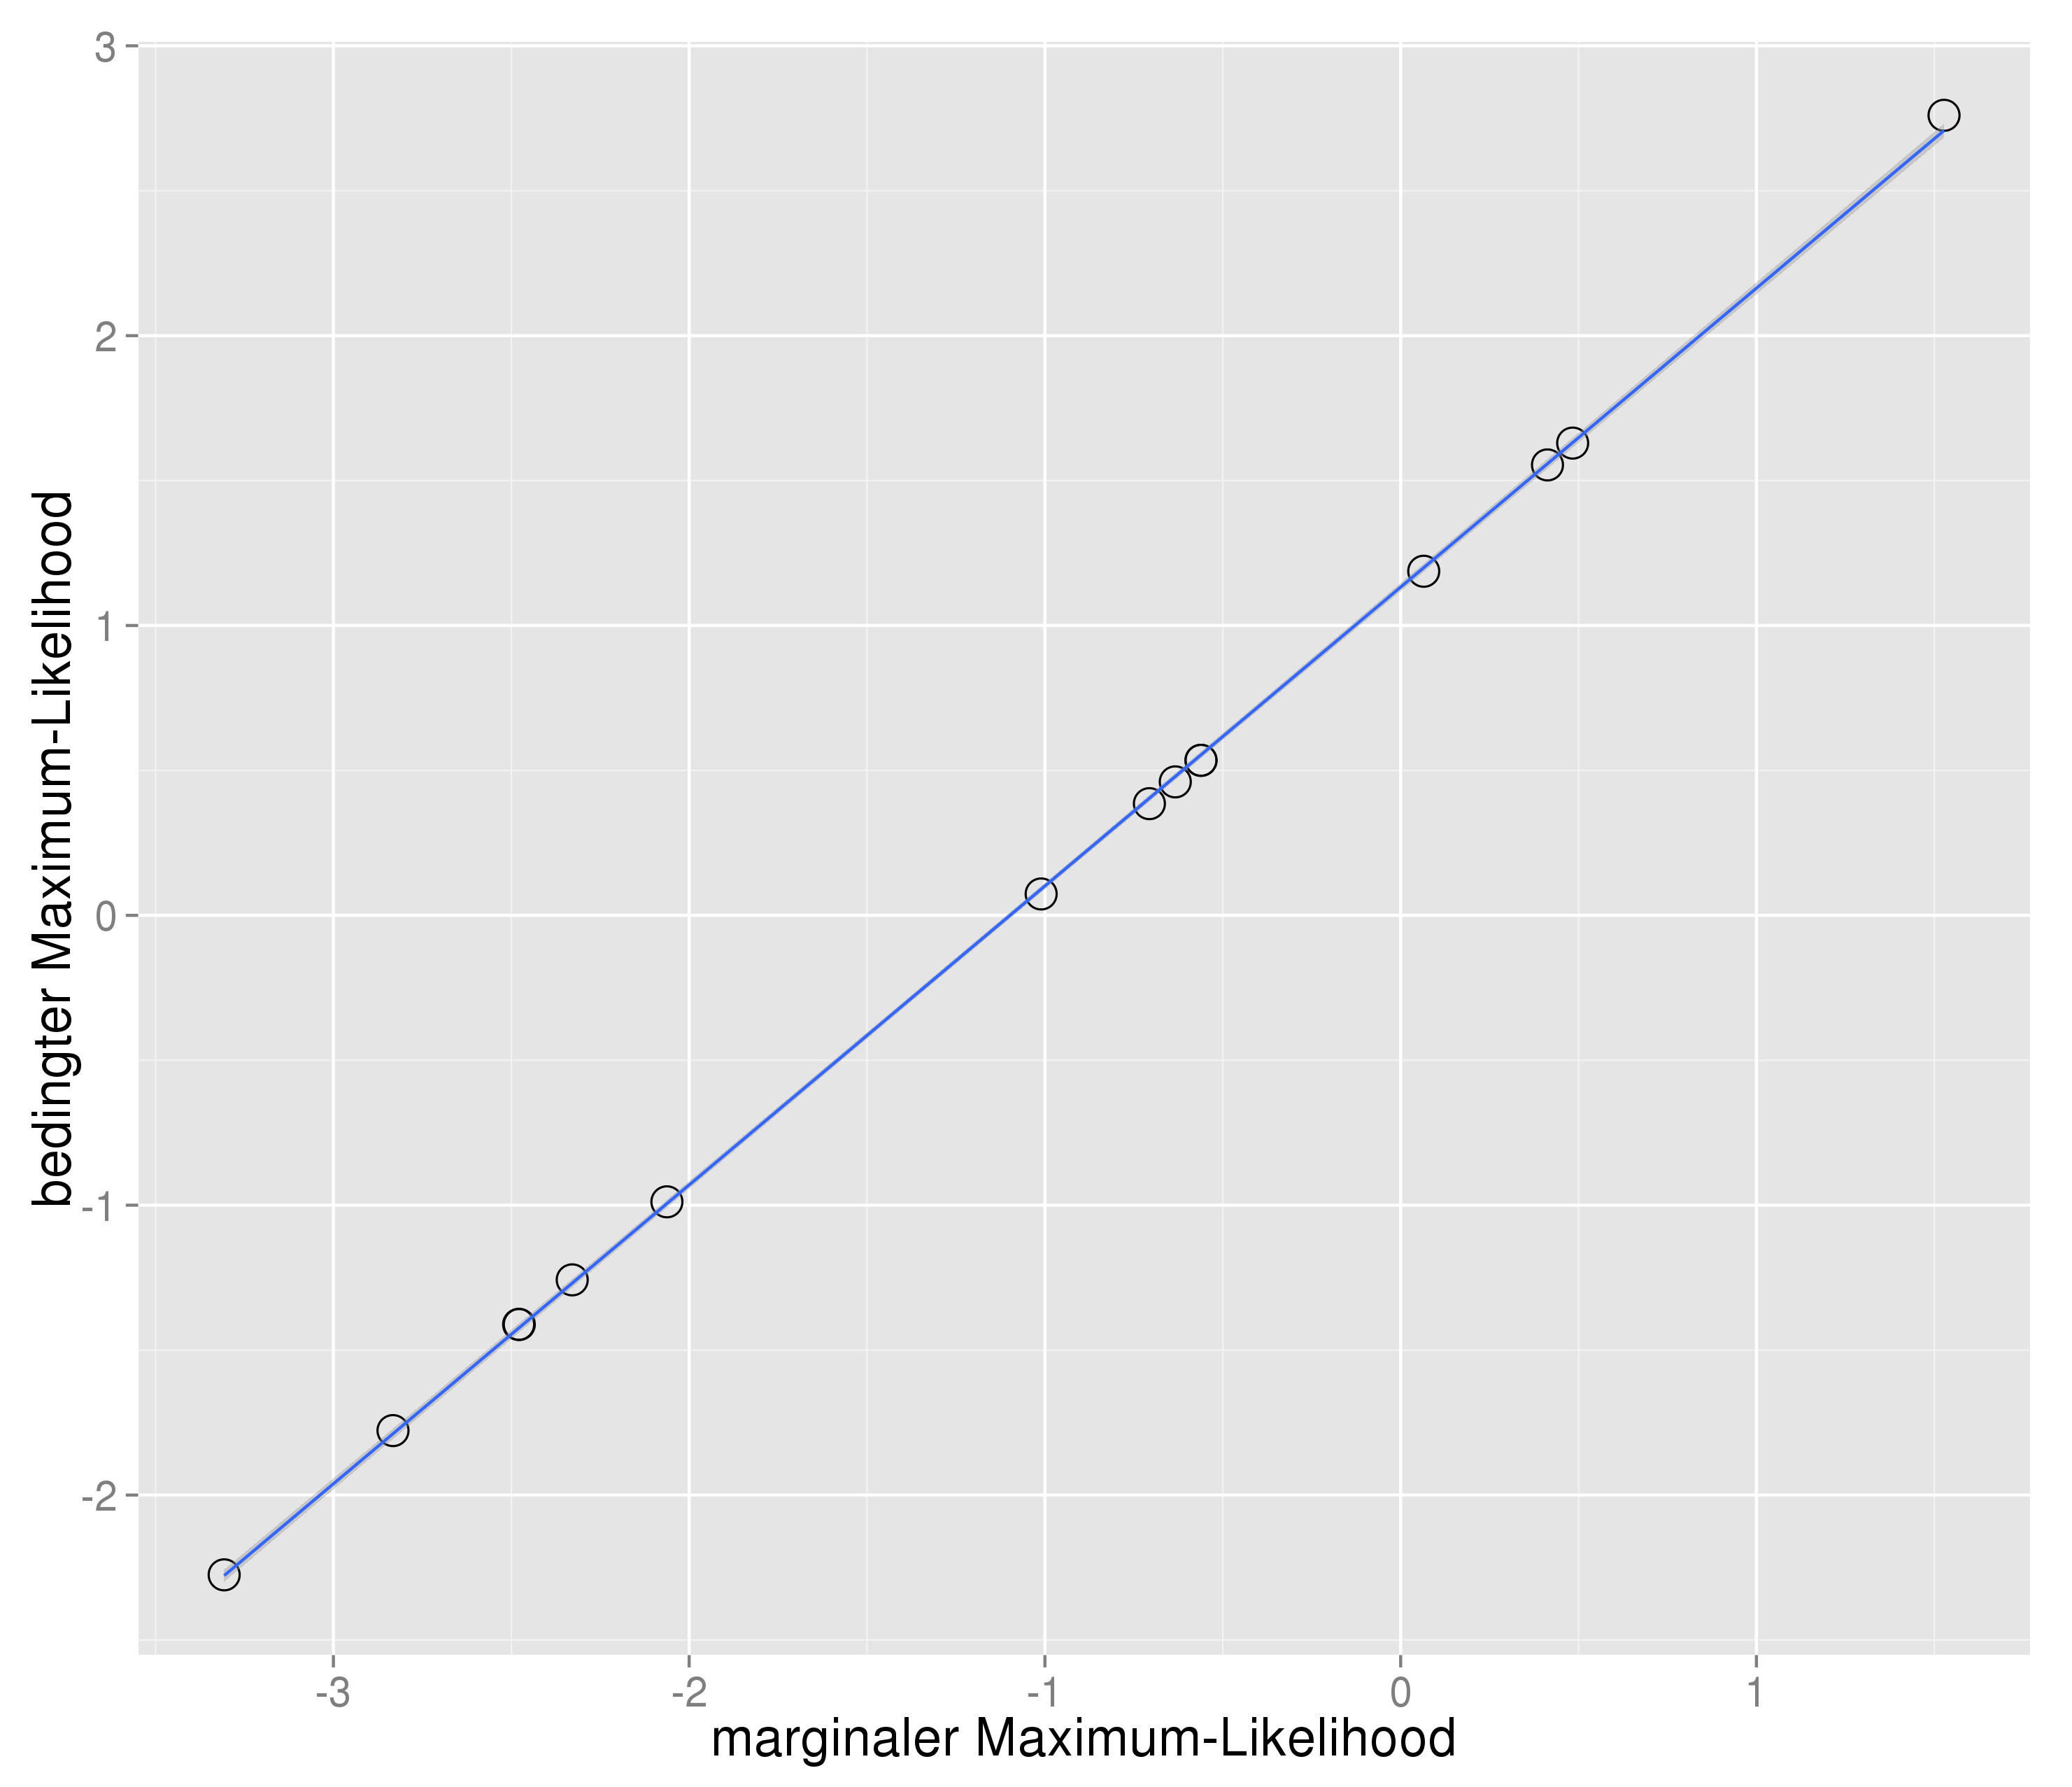
\includegraphics[width=0.7\linewidth]{graphics/RaschVergleich.png}
\caption{Vergleich des Rasch Modells mit der bedingten Maximum-Likelihood-Schätzung und der marginalen Maximum-Likelihood-Schätzung. Da alle Punkte auf einer Geraden liegen, gibt es keinen Unterschied zwischen den unterschiedlichen Schätzmethoden für den vorliegenden Datensatz der 15 unbedingten Qualitätsstandards.  }
\label{fig:RaschVergleich}
\end{figure}

\github{http://git.io/FRxZ}


\subsection{Modellkontrolle des Rasch-Modells}

Um das Rasch Modell zu Validieren wurde das Modell mit Hilfe des Andersens Likelihood-Quotienten Test validiert. Für alle 15 Qualitätsstufen führte dies zu Problemen und der Test konnte nicht durchgeführt werden. Nachdem die Qualitätsstufen vier und fünf entfernt wurden, konnte das reduzierte Modell validiert werden. Als Splitkriterium wurde der Mittelwert der Personen-Randsummen verwendet. 

Der p-Wert des Andersens Likelihood-Quotienten Test beträgt $p=0.14$. Daher liegt jetzt keine signifikante Modellverletzung vor, die Aufgaben Parameter unterscheiden sich nicht signifikant für Personen mit niedrigen und hohen Randsummen. In der Grafik \ref{fig:RaschKontrolle} sind die Resultate des Tests grafisch dargestellt. Es ist ersichtlich, dass keine Aufgabe das Modell verletzt, da die 95\%-Konfidenz-Regionen alle die Diagonale berühren.


\begin{figure}[htbp]

\centering
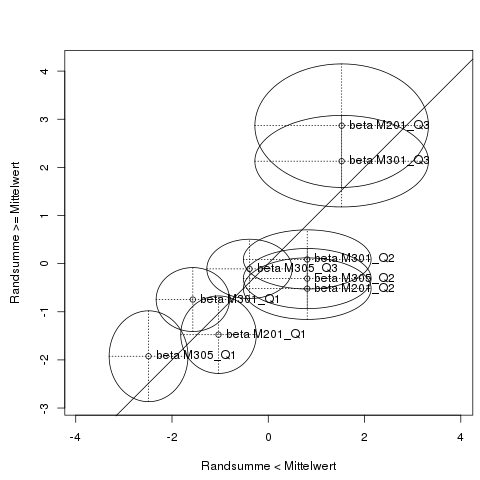
\includegraphics[width=0.8\linewidth]{graphics/GOFQ.png}
\caption{Modellkontrolle des Rasch-Modells: kein Qualitätsstandard hat eine signifikante Abweichung von der Diagonalen, daher gibt es keine signifikanten Unterschiede für Personen mit niedrigen und hohen Randsummen in den Qualitätsstandard. }
\label{fig:RaschKontrolle}
\end{figure}

Zusätzlich wurden die Qualitätsstandards mit dem Wald-Test überprüft. Damit können Qualitätsstandard, welche einen signifikanten Unterschied habe, identifiziert werden. In Tabelle \ref{tab:WaldTest} befinden sich die p-Werte des Wald-Test für die einzelnen Qualitätsstandards.

\begin{table}[htbp]
  \centering
\begin{tabular}{ccccccccccc}
\toprule
 \multicolumn{3}{c}{Test 201} &&  \multicolumn{3}{c}{Test 301}&&  \multicolumn{3}{c}{Test 305}\\ 
 Q1 & Q2 & Q3 && Q1 & Q2 & Q3 && Q1 & Q2 & Q3  \\ 
\midrule
  0.44 & 0.08 & 0.24 && 0.11 & 0.33 & 0.56 && 0.38 & 0.14 & 0.61   \\ 

\bottomrule
\end{tabular} 
  \caption{p-Werte des Wald-Tests für die Qualitätsstandards, mit dem Mittelwert der Personen-Randsummen als Splitkriterium. Keine dieser p-Werte liegt unter halb von $0.05$ daher gibt es keine signifikanten Unterschiede in den Qualitätsstandards }
  \label{tab:WaldTest}
\end{table}

\github{http://git.io/FE3m}

\subsection{Unterschied in den Qualitätsstandards}

Nachdem das Modell kontrolliert wurde soll nun überprüft werden ob es einen Unterschied in den Qualitätsstandards zwischen den einzelnen Test gibt.


  
 \begin{figure}[htp]
 \centering
 \begin{subfigure}{0.49\textwidth}
   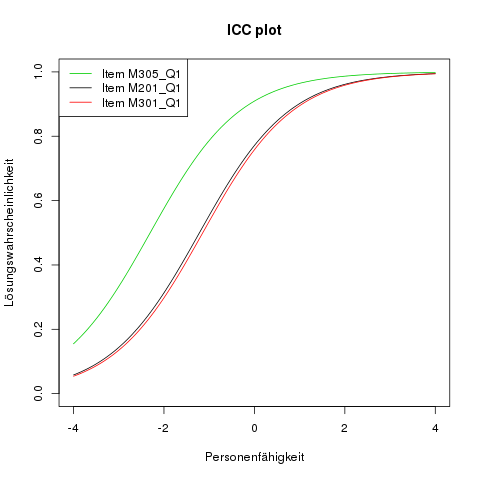
\includegraphics[width=1.0\linewidth]{graphics/ICCQ1.png}
   \caption{ICC Plot für Qualitätsstandard 1}
   \label{fig:ICCQ1}
 \end{subfigure}
 \begin{subfigure}{0.49\textwidth}
   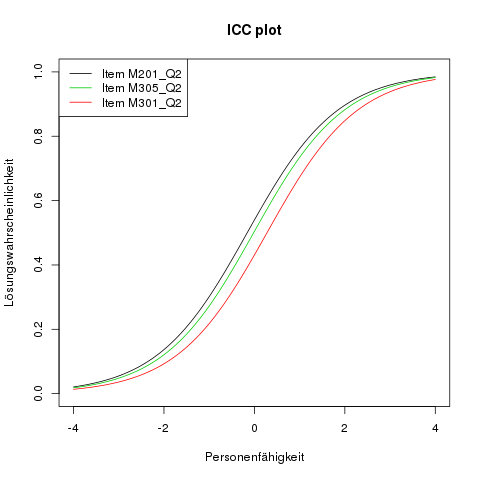
\includegraphics[width=1.0\linewidth]{graphics/ICCQ2.png}
   \caption{ICC Plot für Qualitätsstandard 2}
   \label{fig:ICCQ2}
 \end{subfigure}
 \end{figure}
 \begin{figure}[htbp]
 \ContinuedFloat % continue from previous page
 \centering
 \begin{subfigure}{0.49\textwidth}
   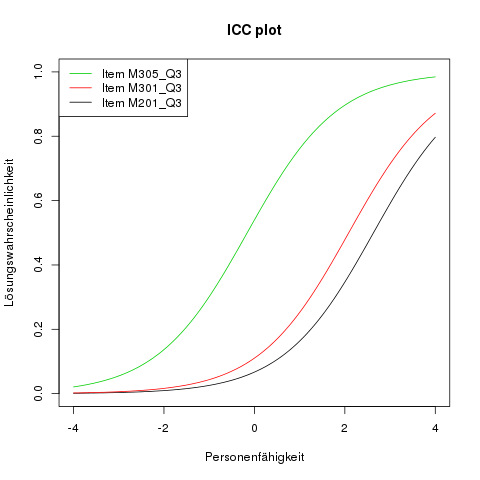
\includegraphics[width=1.0\linewidth]{graphics/ICCQ3.png}
   \caption{ICC Plot für Qualitätsstandard 3}
   \label{fig:ICCQ3}
 \end{subfigure}
 \begin{subfigure}{0.49\textwidth}
   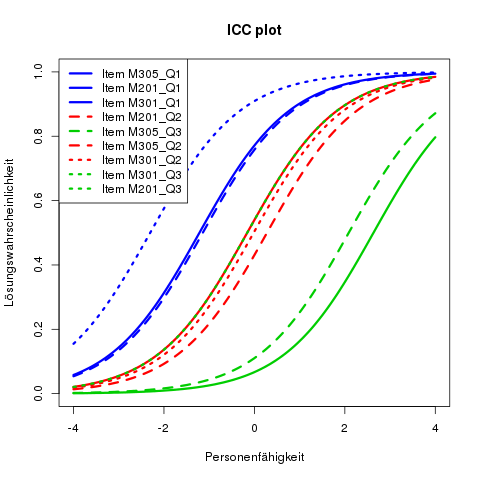
\includegraphics[width=1.0\linewidth]{graphics/ICCQ123.png}
   \caption{ICC Plot für Qualitätsstandard 1,2 und 3}
   \label{fig:ICCQ123}
 \end{subfigure}
 
 \caption{Aufgabencharakteristische Kurven für die Qualitätsstandards 1,2 und 3 für alle drei Tests.}
 \label{fig:corLev}
 \end{figure}
 
 \begin{figure}[htbp]
 
 \centering
 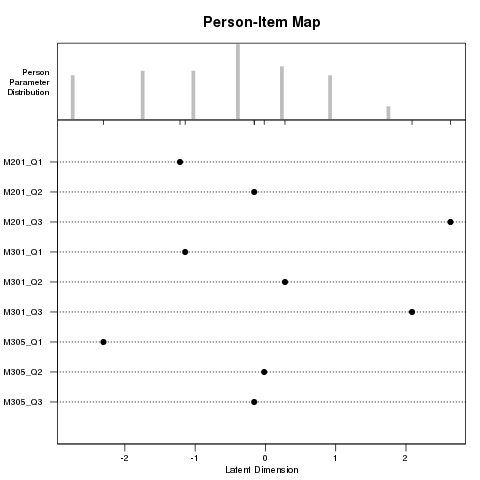
\includegraphics[width=0.8\linewidth]{graphics/PersonItemMap.png}
 \caption{Person-Item-Map auf welcher die Verteilung der Personen basierend auf der latenten Skala ersichtlich ist und die Lage der Aufgaben-Parameter auf der latenten Skala. }
 \label{fig:PersonItemMapQ}
 \end{figure}
 
 In Tabelle \ref{tab:betaQ} finden sich die Aufgaben-Parameter $\beta_j$ der einzelnen Qualitätsstandards.
 
 \begin{table}[htbp]
   \centering
 \begin{tabular}{ccccccccccc}
 \toprule
  \multicolumn{3}{c}{Test 201} &&  \multicolumn{3}{c}{Test 301}&&  \multicolumn{3}{c}{Test 305}\\ 
  Q1 & Q2 & Q3 && Q1 & Q2 & Q3 && Q1 & Q2 & Q3  \\ 
 \midrule
   1.215 & 0.159 & -2.633 && 1.142 & -0.278 & -2.086 && 2.305 & 0.017 & 0.159   \\ 
 
 \bottomrule
 \end{tabular} 
   \caption{Aufgaben-Parameter $\beta_j$ für die einzelnen Qualitätsstandards. }
   \label{tab:betaQ}
 \end{table}